In this section, we want to motivate the advantage of the numerical smoothing idea in the context of MLMC method. For this aim we consider two examples: i) the first one is for computing the price of a digital option under GBM and Heston models (see Section \ref{sec: MLMC for digital options}) , and ii) the second example is for approximating a density function for dynamics following  GBM and Heston models (see Section \ref{sec: MLMC for approximating densities and greeks}). The idea and results of Section \ref{sec: MLMC for digital options}  can be generalized to i)  any kind of option having low regularity in the payoff function, or  ii) for computing distribution functions, since it involves the indicator function.  On the other hand, examples in Section \ref{sec: MLMC for approximating densities and greeks}  have two important applications: i) computing density functions which involves the use of Dirac delta functions and which is hard to approximate its expectation using MLMC due to the infinite variance, and ii) computing Greeks for an option with a non smooth payoff function.
\subsection{Our contributions to the literature}
Usually, for such  tasks, standard MLMC will fail or not have the optimal performance, due to the singularity present in the delta or the indicator functions, implying either high variance or kurtosis for the MLMC estimator. In the literature, few works tried to address this issue. For instance,
\begin{enumerate}
\item Avikainen in \cite{avikainen2009irregular}, and Giles, Higham, and Mao in \cite{giles2009analysing} used MLMC for such a task without smoothing.
\item On the other hand, a second approach  was suggested in  \cite{giles2008improved,giles2013numerical}, that used implicit smoothing based on the use of conditional expectations. There are two potential issues  with this second approach: i) In general cases, one may have dynamics where it is not easy to derive an  analytic expression for the conditional expectation and ii) This approach used a higher order scheme, that is the Milstein scheme, to improve the strong order of convergence, and consequently the complexity of the MLMC estimator. Such a scheme becomes very computationally expensive for higher dimensional dynamics. Different non smooth payoff functions were considered in \cite{giles2008improved,giles2013numerical} (Asian, barrier, digital)  but the only considered dynamics were under the GBM model.
\item In \cite{giles2015multilevel}, the authors suggested a different approach based on parametric smoothing.  In fact, they carefully constructed a regularized version of the QoI, based on a 
regularization parameter that depends on the weak and strong convergence rates and also  the tolerance requirement.  This approach, despite offering better performance for the MLMC estimator and a better setting for theoretical analysis, it has the practical disadvantage consisting in the difficulty of generalizing it to cases where there is no prior knowledge of the the convergence rates (that is they need to be estimated numerically), and also for each error tolerance, a new  regularization parameter needs to be computed. Note also that all the numerical examples in \cite{giles2015multilevel} were based on the GBM dynamics.
\end{enumerate}    

In this work, we address a similar problem and  propose an alternative approach that is  based on numerical smoothing. Our approach compared to previous mentioned works, has the following advantages
\begin{enumerate}
\item It can be easily applied to cases where one can not apply analytic smoothing.
\item We obtain similar  rates of strong convergence and MLMC complexity  as in  \cite{giles2008improved,giles2013numerical}, without the need to use higher order schemes such as Milstein scheme.
\item Our approach is parameter free compared to that of  \cite{giles2015multilevel}. Therefore, in practice it is much easier to apply for any dynamics and QoI.
\item Compared to \cite{giles2008improved,giles2013numerical,giles2015multilevel}, we add numerical results for the Heston model were discretization is needed unlike the GBM dynamics which is considered here as a toy example.
\end{enumerate} 

\subsection{MLMC for digital options}\label{sec: MLMC for digital options}
In this section, we motivate the idea of using the numerical smoothing idea to compute option prices for non smooth payoff function. For illustration, we consider  the price of the digital option, that is we want to approximate
\begin{align}
\expt{g(X)}=\expt{\mathbf{1}_{X>K}},
\end{align}
where $K$ is the strike. 

In this kind of problems, we have a very well known issue related to observing high kurtosis problem for very fine discretization levels of the MLMC method. We try in the following Section to explain this issue.
\subsubsection{High kurtosis issue}\label{sec:General motivation}
Let $g$ denote a random variable, and let $g_{\ell}$ denote the corresponding level $\ell$ numerical approximation. We also define $Y_{\ell}$ to be
\[
 Y_{\ell}=\begin{cases}
               g_0,\quad \ell=0\\
               g_{\ell}-g_{\ell-1},\quad \ell>1.
            \end{cases}
\]
and the multilevel estimator 
\begin{equation}
Y=\sum_{\ell=0}^L \expt{Y_{\ell}}
\end{equation}
The MLMC approach needs a good estimate for $V_{\ell}=\text{Var}[Y_{\ell}]$. When the number of samples $N$ is large, the standard deviation of the sample variance for a random variable $X$ with zero mean is approximately $\sqrt{(\kappa-1)/N} \expt{X^2}$ where the kurtosis $\kappa$ is defined as
\begin{align}\label{eq:Kurtosis}
\kappa = \frac{\expt{X^4}}{(\expt{X^2})^2}.
\end{align}  
Hence $\Ordo{\kappa}$ samples are required to obtain a reasonable estimate for the variance.  An extreme, but important, example is when $g$ always takes the value $0$ or $1$. In this case we have
\[
X \equiv g_{\ell}-g_{\ell-1}=\begin{cases}
               1,\quad \text{probability} \quad p\\
               -1,\quad \text{probability}\quad q\\
               0,\quad \text{probability} \quad 1-p-q
            \end{cases}
\]
if $p,q \ll 1$, then $\expt{X} \approx0$  and $\kappa=(p+q)^{-1}\gg 1$. Therefore, many samples are required for a good estimate of $V_{\ell}$; otherwise, we may get all $X(n)=0$, which will give an estimated variance of zero. Furthermore, the kurtosis will become worse as $\ell \rightarrow \infty$ since $p,q \rightarrow0$ due to weak convergence.

\subsubsection{Summary of results for the digital option}\label{sec:Summary of results for the digital option}
In this Section, we try to summarize the obtained results for approximating the price of a digital option using MLMC with and without numerical smoothing for two models: the GBM model (see Table \ref{table:Summary of our numerical results digital GBM.} and  detailed results in Section \ref{sec:Digital options under the GBM model}) and the Heston model (see Table \ref{table:Summary of our numerical results digital Heston.} and  detailed results in Section \ref{sec:Digital option under the Heston model}). From these tables, we can see two main results
\begin{enumerate}
\item The significant reduction of the kurtosis at the finest levels, $\kappa_{L}$, of MLMC algorithm when using numerical smoothing. In fact, the kurtosis is reduced by a factor of $200$ for the GBM dynamics and by a factor of $28$  for the Heston model.
\item Numerical smoothing has significantly improved the strong rate $\beta$ for the example under GBM model from $\beta=1/2$ to $\beta=1$ resulting in reducing the order of MLMC complexity from $\Ordo{TOL^{-2.5}}$ to $\Ordo{TOL^{-2} \left(\log(TOL)\right)^2}$. On the other hand, numerical smoothing also improved  the strong rate for  the example under Heston model from $\beta=2/3$ to $\beta=9/10$ for the full truncation scheme resulting in an improvement of the MLMC complexity from  $\Ordo{TOL^{-2.5}}$ to $\Ordo{TOL^{-2}}$. Note that full truncation scheme performed better than the smooth scheme when coupled with numerical smoothing.
\end{enumerate}

\FloatBarrier
\begin{table}[!h]
	\centering
	\begin{small}
	\begin{tabular}{l*{4}{c}r}
	\toprule[1.5pt]
		Method      &   $\kappa_{L}$  & $\alpha$  & $\beta$  &  $\gamma$   & Complexity \\
		\hline
			Without smoothing & $621$& $1$ & $1/2$ & $1$&  $\Ordo{TOL^{-2.5}}$ \\	
              \hline
           With numerical smoothing   & $3$& $1$ & $1$ & $1$&  $\Ordo{TOL^{-2} \left(\log(TOL)\right)^2}$ \\
		\bottomrule[1.25pt]
	\end{tabular}
\end{small}
	\caption{Summary of the MLMC numerical results observed for  computing the price of the digital option under GBM model. $\kappa_{L}$ is the kurtosis at the finest levels of MLMC with $\Delta t_{L}=T.2^{-10}$, $(\alpha,\beta,\gamma)$ are weak, strong and work rates respectively. $TOL$ is the user selected  MLMC  tolerance. These results correspond to Figures \ref{fig:euler_digital_without_smoothing} and \ref{fig:euler_digital_with_smoothing}.}
	\label{table:Summary of our numerical results digital GBM.}
\end{table}
\FloatBarrier

\begin{table}[!h]
	\centering
	\begin{small}
	\begin{tabular}{l*{4}{c}r}
	\toprule[1.5pt]
		Method      &     $\kappa_{L}$ & $\alpha$   &  $\beta$  &  $\gamma$   & Complexity \\
		\hline
			Without smoothing $+$ the full truncation scheme  & $746$ & $1$  &  $3/5$&  $1$&  $\Ordo{TOL^{-2.4}}$\\	
              \hline 
            With  smoothing  $+$ smooth scheme & $6$ & $1$  &  $4/5$ & $1$ &  $\Ordo{TOL^{-2.2}}$\\	
               \hline
%           With  smoothing $+$ full truncation scheme $(\Delta t_0=2^{-2}),L=4(\Delta t_L=2^{-6}))$ & $6$ & $1/2$  &  $3/4$&  $1$ &  $\Ordo{TOL^{-2.5}}$\\
            With  smoothing $+$ full truncation scheme  & $5$ & $2.2$  &  $4/5$&  $1$ &  $\Ordo{TOL^{-2.1}}$\\	 
		\bottomrule[1.25pt]
	\end{tabular}
\end{small}
	\caption{Summary of the MLMC numerical results observed for  computing the price of the digital option under Heston model. $\kappa_{L}$ is the kurtosis at the finest levels of MLMC with $\Delta t_{L}=T.2^{-10}$, $(\alpha,\beta,\gamma)$ are weak, strong and work rates respectively. $TOL$ is the user selected  MLMC  tolerance.  These results correspond to Figures \ref{fig:euler_digital_Heston_without_smoothing}, \ref{fig:euler_digital_Heston_with_smoothing_OU} and \ref{fig:euler_digital_Heston_with_smoothing_FT}.}
	\label{table:Summary of our numerical results digital Heston.}
\end{table}
\FloatBarrier
\subsubsection{Digital options under the GBM model}\label{sec:Digital options under the GBM model}
Using similar idea introduced in Section \ref{sec:The discretized 1D Black-Scholes}, we can show that
\begin{align}
\expt{g(X)}&=\expt{\mathbf{1}_{X>K}}\nonumber\\
&=\expt{1-\Phi(y^\ast(K))},
\end{align}
where $y^\ast(K)$ is the kink location obtained by solving numerically 
$$X(T; y^\ast(K), \mathbf{z}_{-1})=K,$$
where  $\mathbf{z}$ is $N-1$ Gaussian random  vector ($N$ is the number of time steps) used for Brownian bridge construction, and $\Phi$ is the cumulative Gaussian distribution function.

As an illustration, we choose the digital option of GBM asset with parameters: $S_0=K=100$, $T=1$, $r= 0$, and   $\sigma=0.2$, and we compare MLMC results with the original payoff function (without numerical smoothing), given by Figure \ref{fig:euler_digital_without_smoothing},  and MLMC results after applying our numerical smoothing idea, given by Figure \ref{fig:euler_digital_with_smoothing}. From these two Figures we have the following conclusions:
\begin{enumerate}
\item The numerical smoothing has improved the rate of strong convergence from $1/2$ (without smoothing) to $1$ after doing the numerical smoothing (compare both top left plots in Figures \ref{fig:euler_digital_without_smoothing} and Figure \ref{fig:euler_digital_with_smoothing}).
\item The numerical smoothing has also dropped significantly the kurtosis at the finest level, $\kappa_L$, by a factor $200$, this is can be seen clearly by comparing the middle right plots in both Figures \ref{fig:euler_digital_without_smoothing} and Figure \ref{fig:euler_digital_with_smoothing}. We stress that this is an important improvement, since one needs $\Ordo{\kappa}$ samples  to obtain a reasonable estimate for the variance (see Section \ref{sec:General motivation}).  
\item Finally, improving the strong error rate after using the numerical smoothing, resulted in an improvement of the complexity rate going from $TOL^{-2.5}$ for the case without smoothing to  $TOL^{-2}$, where $TOL$ is a prescribed tolerance, for the case where MLMC is coupled with numerical smoothing (compare the bottom right plots in Figures \ref{fig:euler_digital_without_smoothing} and \ref{fig:euler_digital_with_smoothing}).
\end{enumerate}
\FloatBarrier
\begin{figure}[htb]
	\centering 
	\begin{subfigure}{0.5\textwidth}
		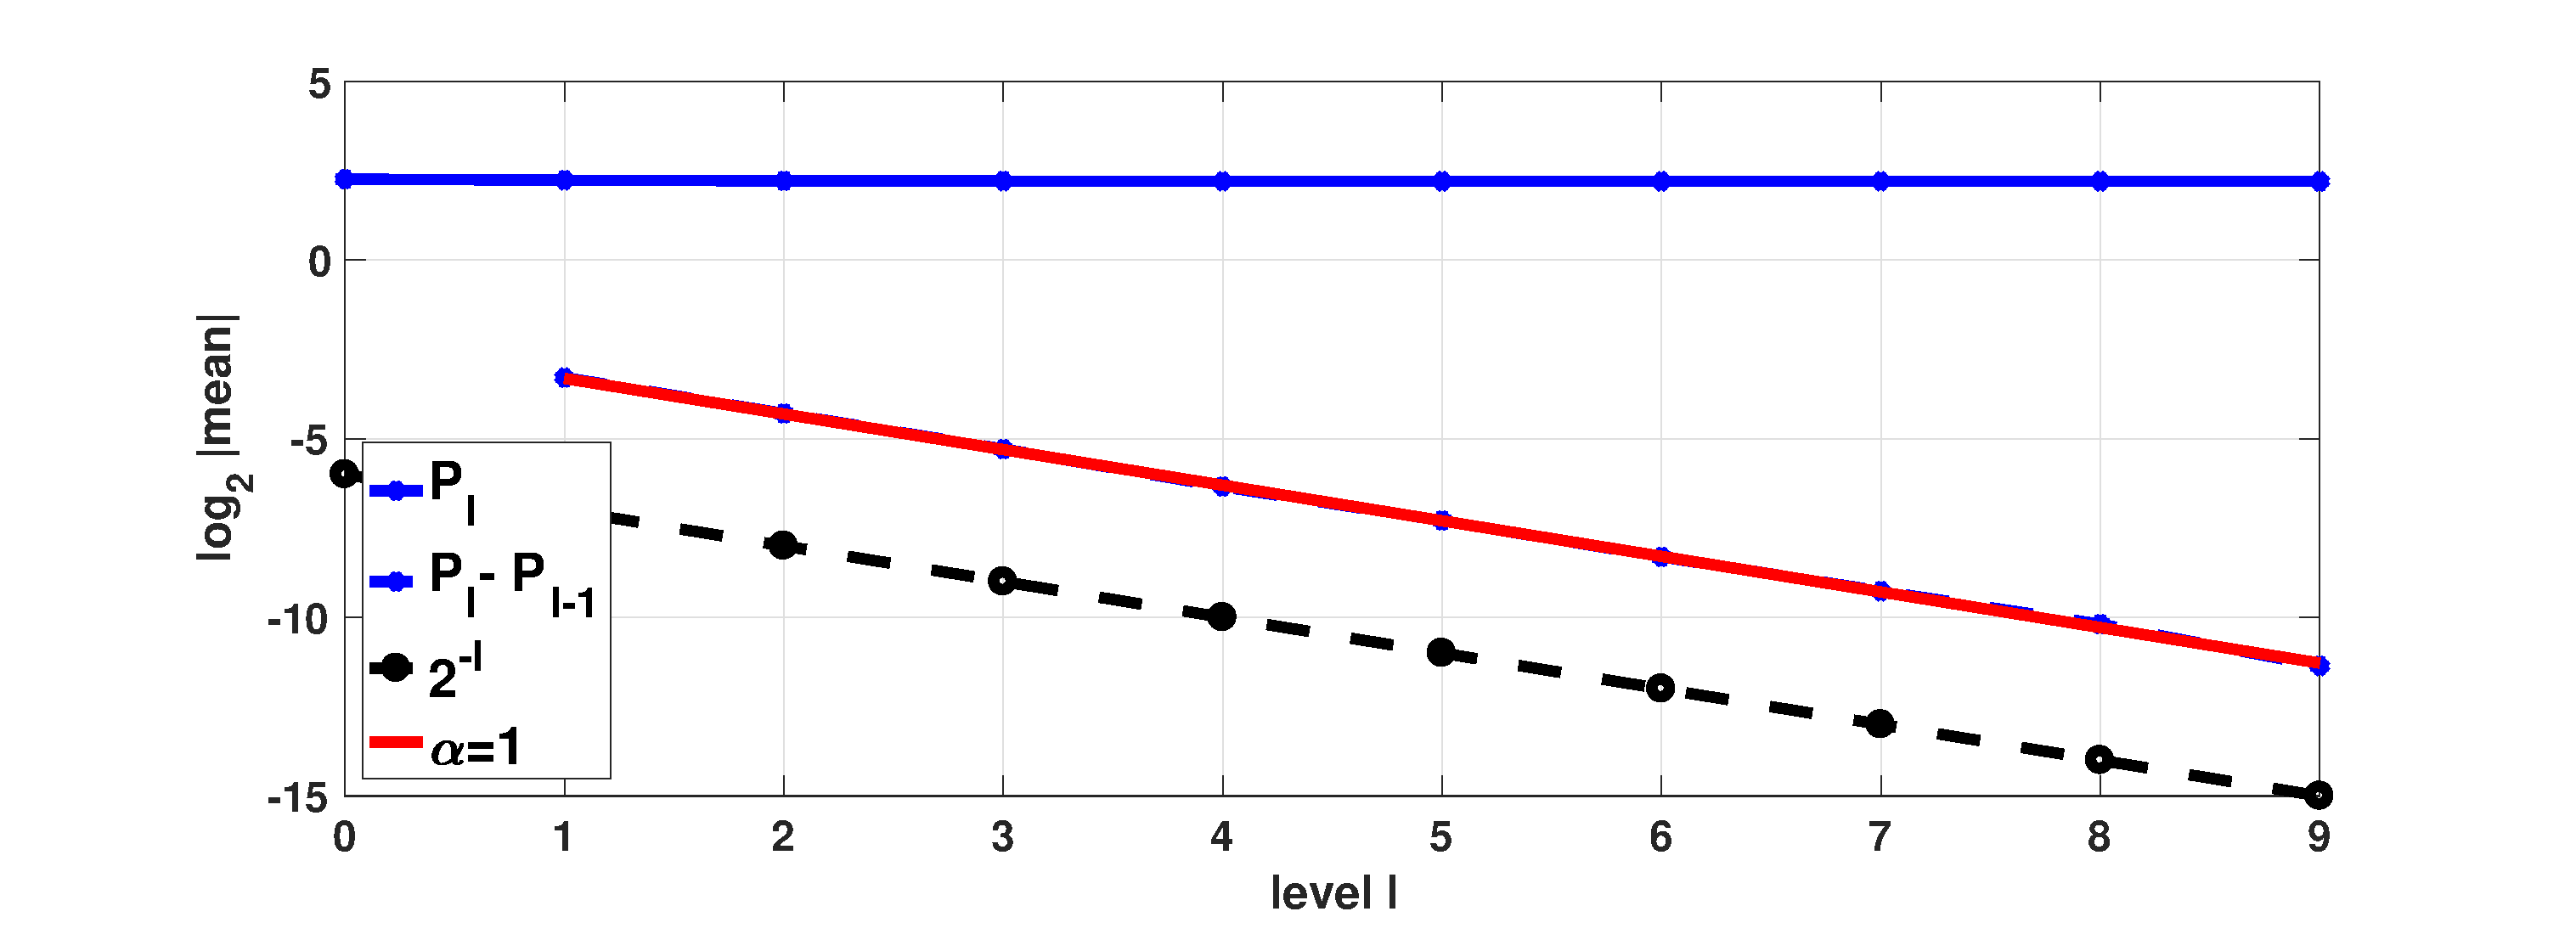
\includegraphics[width=\linewidth]{./figures/MLMC_binary_GBM_opt/without_smoothing/digital_option_set1_L_0_2_steps_L_9_N_10_7_weak}
		\caption{}
		\label{fig:weak_rate_GBM_digital_non_smoothing}
	\end{subfigure}\hfil %% <-- added
	\begin{subfigure}{0.5\textwidth}
		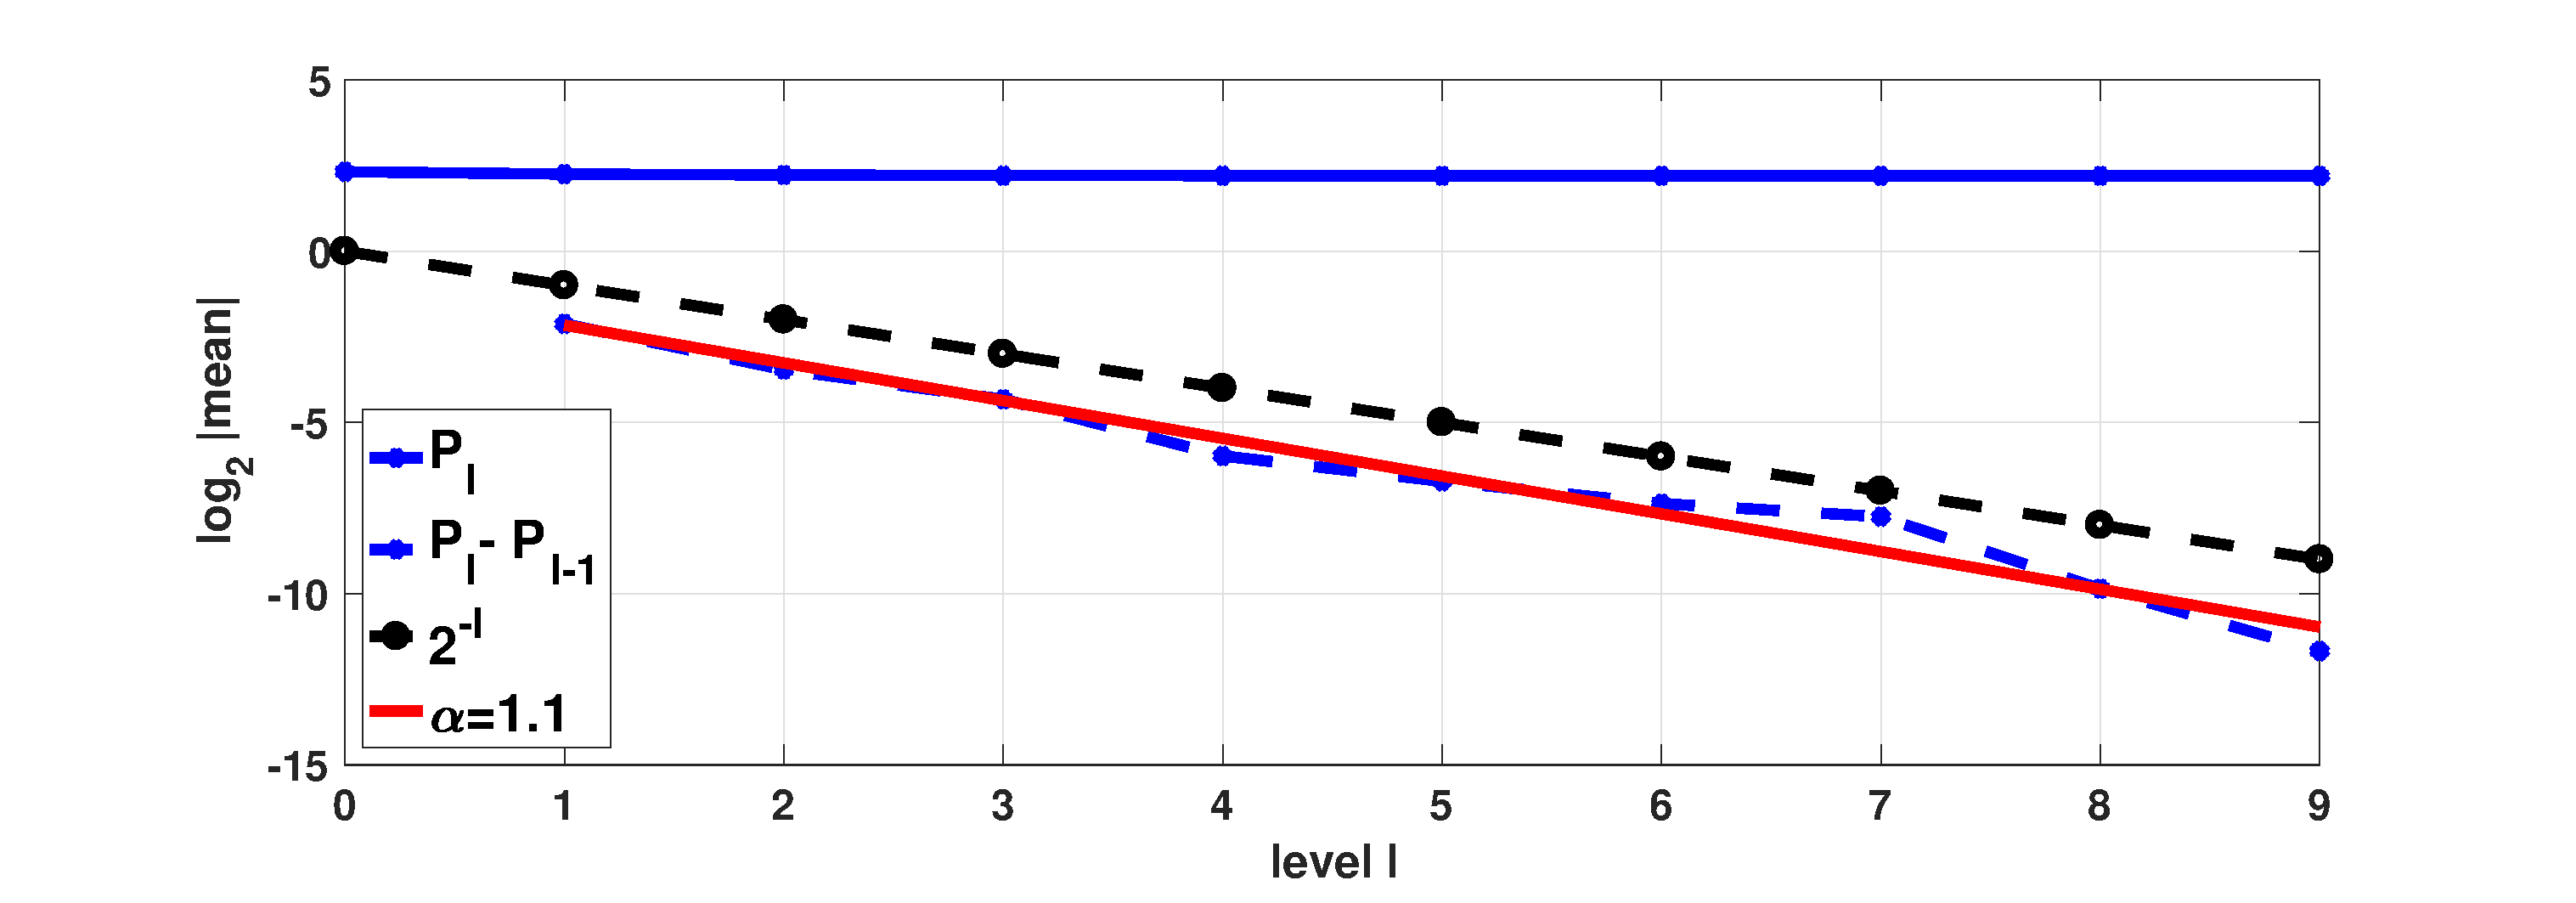
\includegraphics[width=\linewidth]{./figures/MLMC_binary_GBM_opt/with_smoothing/digital_option_set1_L_0_2_steps_L_9_N_10_5_weak}
		\caption{}
		\label{fig:weak_rate_GBM_digital_smoothing}
	\end{subfigure}\hfil 
	\caption{Convergence of the weak error,  $\expt{P_{\ell}-P_{\ell-1}}$. a) MLMC without smoothing, b) MLMC with numerical smoothing using the smooth scheme defined in Section \ref{sec:Discretization of Heston model with the volatility process Simulated using the sum of  Ornstein-Uhlenbeck (Bessel) processes}, c) MLMC with numerical smoothing using the full truncation scheme defined in Section \ref{sec:Discretization of Heston model with a non smooth transformations for the volatility process}. Estimation done with $M=10^7$ samples.}
	\label{fig:weak_rate_GBM_digital}	
\end{figure}
\FloatBarrier

\begin{figure}[htb]
	\centering % <-- added
	\begin{subfigure}{0.5\textwidth}
		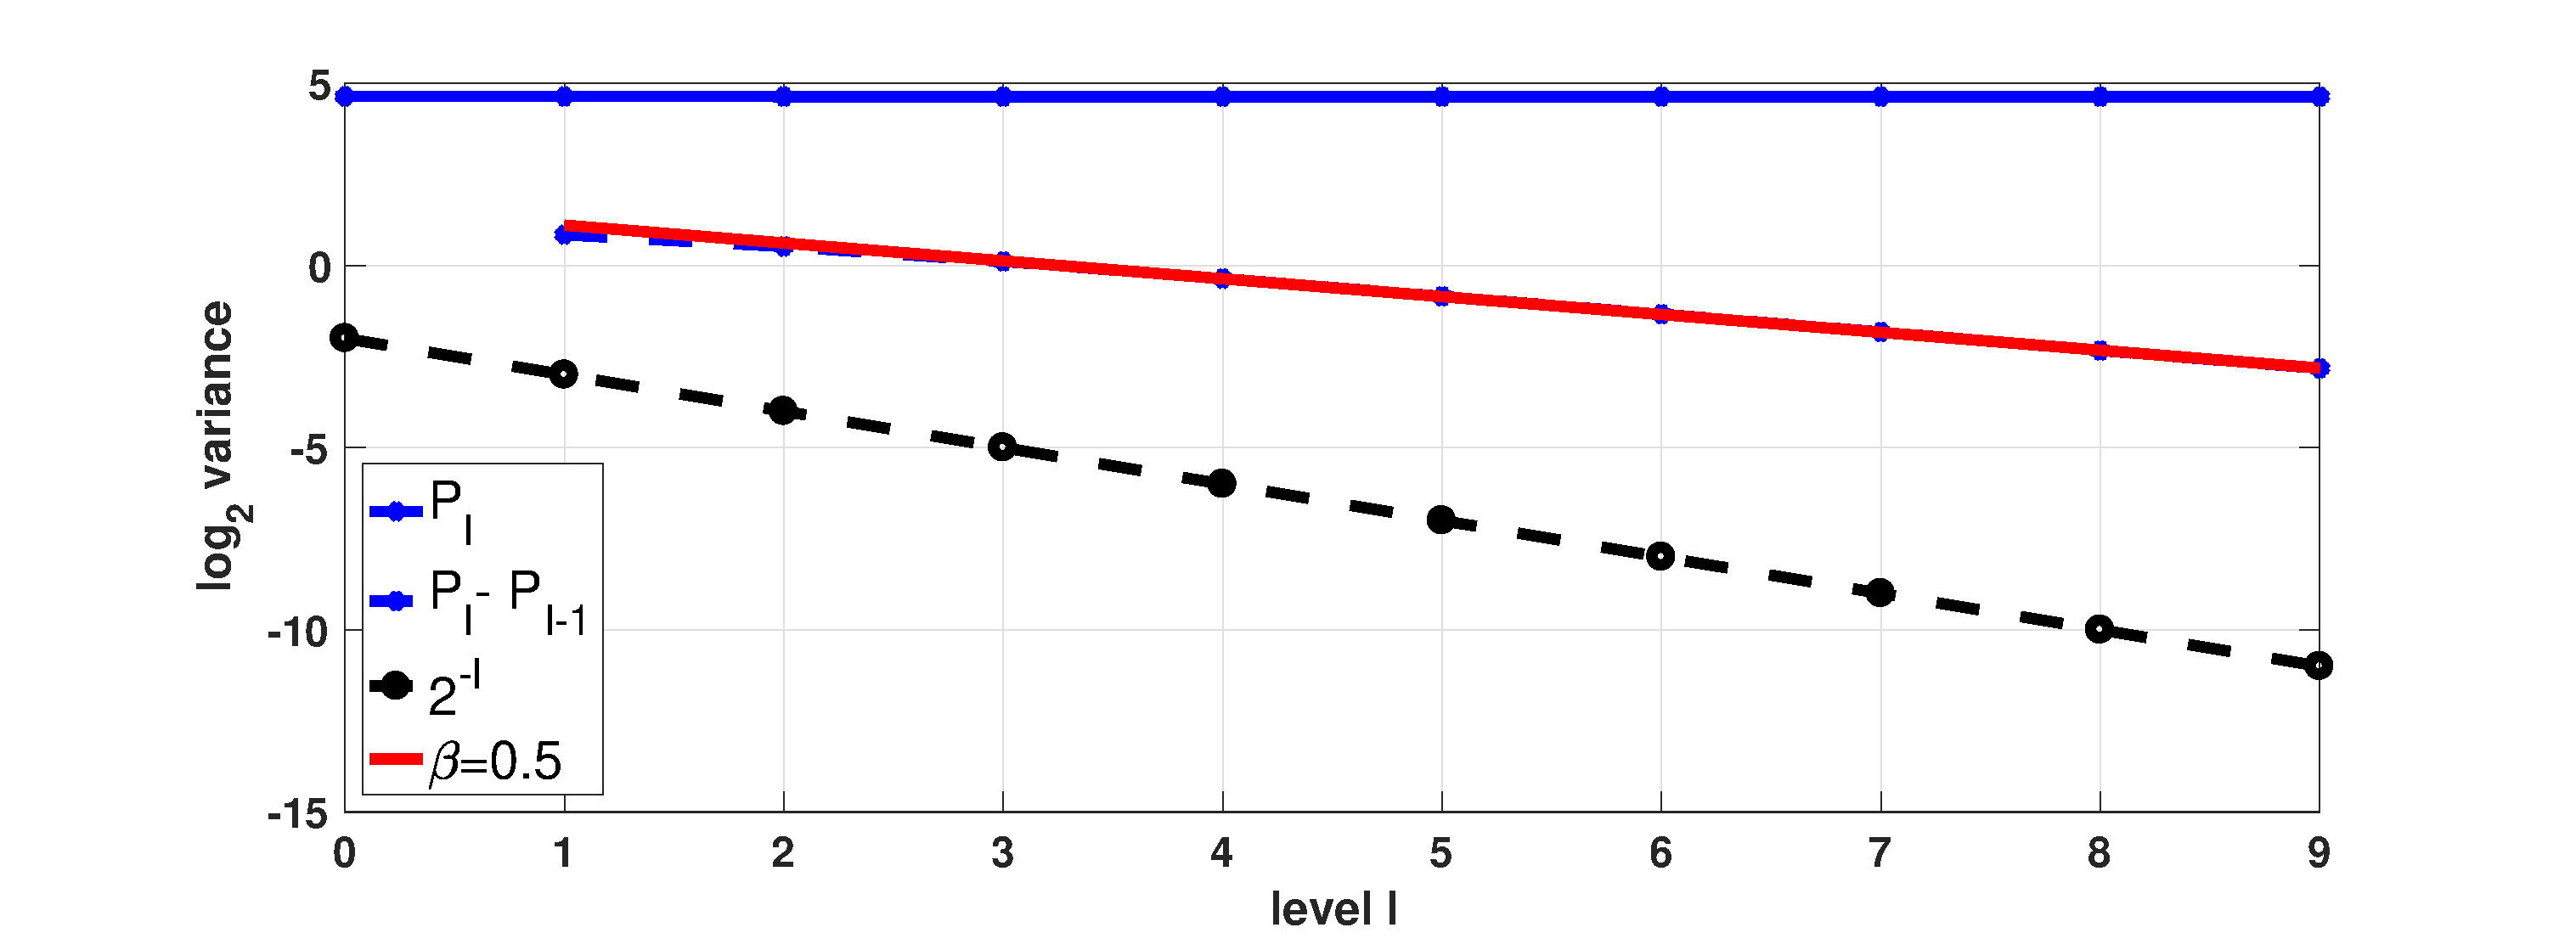
\includegraphics[width=\linewidth]{./figures/MLMC_binary_GBM_opt/without_smoothing/digital_option_set1_L_0_2_steps_L_9_N_10_7_strong}
		\caption{}
		\label{fig:strong_rate_GBM_digital_non_smoothing}
	\end{subfigure}\hfil %% <-- added
	\begin{subfigure}{0.5\textwidth}
		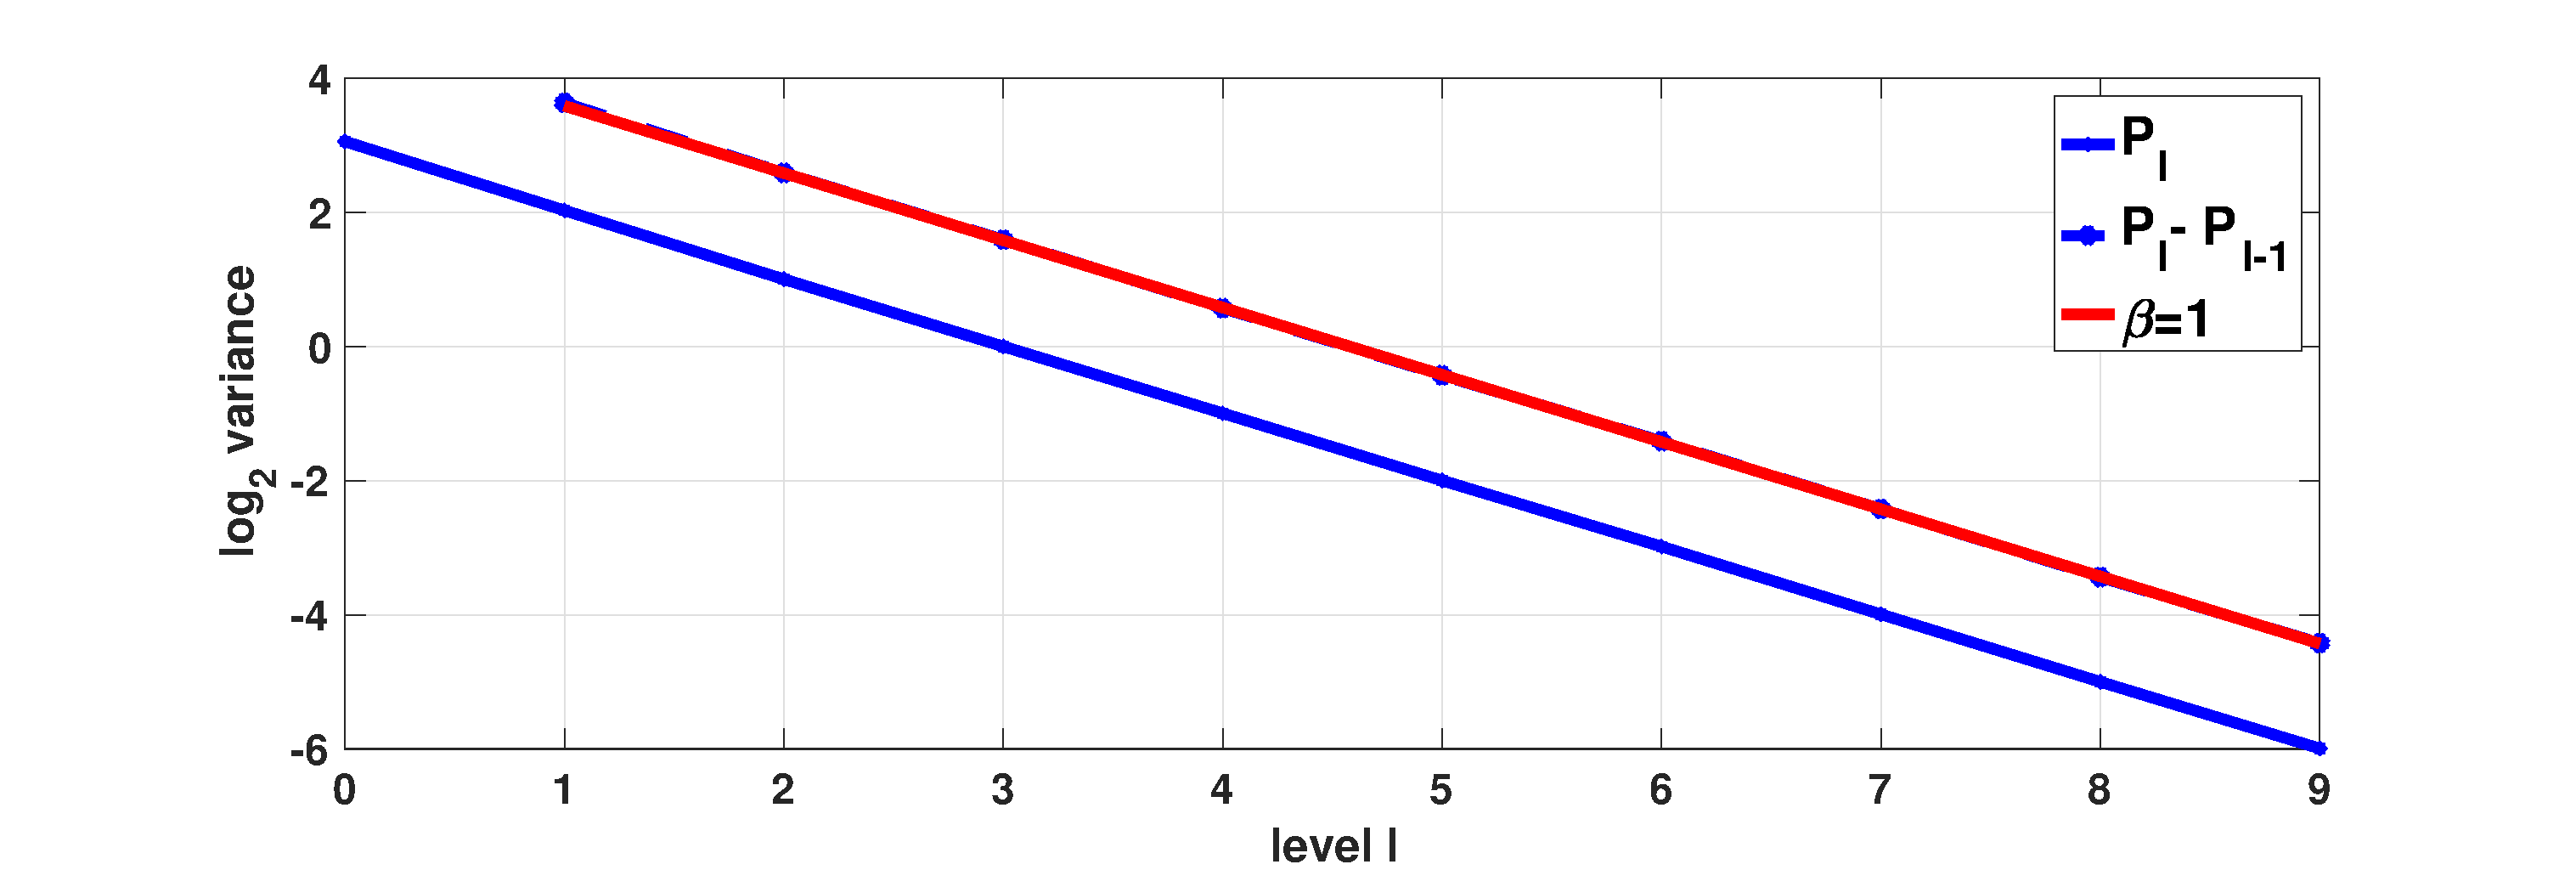
\includegraphics[width=\linewidth]{./figures/MLMC_binary_GBM_opt/with_smoothing/digital_option_set1_L_0_2_steps_L_9_N_10_5_strong}
		\caption{}
		\label{fig:strong_rate_GBM_digital_smoothing}
	\end{subfigure}\hfil 
	\caption{Convergence of  the strong error, $\text{Var}\left[P_{\ell}-P_{\ell-1}\right]$. a) MLMC without smoothing, b) MLMC with numerical smoothing using the smooth scheme defined in Section \ref{sec:Discretization of Heston model with the volatility process Simulated using the sum of  Ornstein-Uhlenbeck (Bessel) processes}, c) MLMC with numerical smoothing using the full truncation scheme defined in Section \ref{sec:Discretization of Heston model with a non smooth transformations for the volatility process}.  Estimation done with $M=10^7$ samples.}
	\label{fig:strong_rate_GBM_digital}	
\end{figure}
\FloatBarrier

%
%\begin{figure}[htb]
%	\centering % <-- added
%	\begin{subfigure}{0.4\textwidth}
%		\includegraphics[width=\linewidth]{./figures/MLMC_binary_Heston_opt/without_smoothing/digital_option_set1_L_0_1_steps_L_6_2_N_10_7/digital_option_set1_L_0_1_steps_L_6_2_N_10_7_complexity}
%		\caption{}
%		\label{fig:complex_rate_hest_digital_non_smoothing_FT}
%	\end{subfigure}\hfil %% <-- added
%	\begin{subfigure}{0.4\textwidth}
%		\includegraphics[width=\linewidth]{./figures/MLMC_binary_Heston_opt/with_smoothing/OU/digital_option_set1_L_0_2_steps_L_5_N_10_7_beta_128/digital_option_set1_L_0_2_steps_L_5_N_10_7_complexity}
%		\caption{}
%		\label{fig:complex_rate_hest_digital_smoothing_OU}
%	\end{subfigure}\hfil %% <-- added
%	\begin{subfigure}{0.4\textwidth}
%		\includegraphics[width=\linewidth]{./figures/MLMC_binary_Heston_opt/with_smoothing/FT/digital_option_set1_L_0_2_steps_L_5_N_10_7_beta_128/digital_option_set1_L_0_2_steps_L_5_N_10_7_complexity}
%		\caption{}
%		\label{fig:strong_rate_hest_digital_smoothing_FT}
%	\end{subfigure}
%	\caption{}
%	\label{fig:complex_rate_hest_digital}	
%\end{figure}
%\FloatBarrier

\begin{figure}[htb]
	\centering % <-- added
	\begin{subfigure}{0.5\textwidth}
		\includegraphics[width=\linewidth]{./figures/MLMC_binary_GBM_opt/without_smoothing/digital_option_set1_L_0_2_steps_L_9_N_10_7_kurt}
		\caption{}
		\label{fig:kurt_GBM_digital_non_smoothing_FT}
	\end{subfigure}\hfil %% <-- added
	\begin{subfigure}{0.5\textwidth}
		\includegraphics[width=\linewidth]{./figures/MLMC_binary_GBM_opt/with_smoothing/digital_option_set1_L_0_2_steps_L_9_N_10_5_kurt}
		\caption{}
		\label{fig:kurt_GBM_digital_smoothing}
	\end{subfigure}\hfil %% <-- added
	\caption{Comparison of the kurtosis $\kappa_{\ell}$, defined in \eqref{eq:Kurtosis} between a) MLMC without smoothing and b) MLMC with numerical smoothing. We can see that the numerical smoothing has dropped significantly the kurtosis at the finest level $L=10$  by a factor  of about $28$.  Estimation done with $M=10^7$ samples.}
	\label{fig:kurt_GBM_digital}	
\end{figure}
\FloatBarrier

	\begin{figure}[h!]
\centering
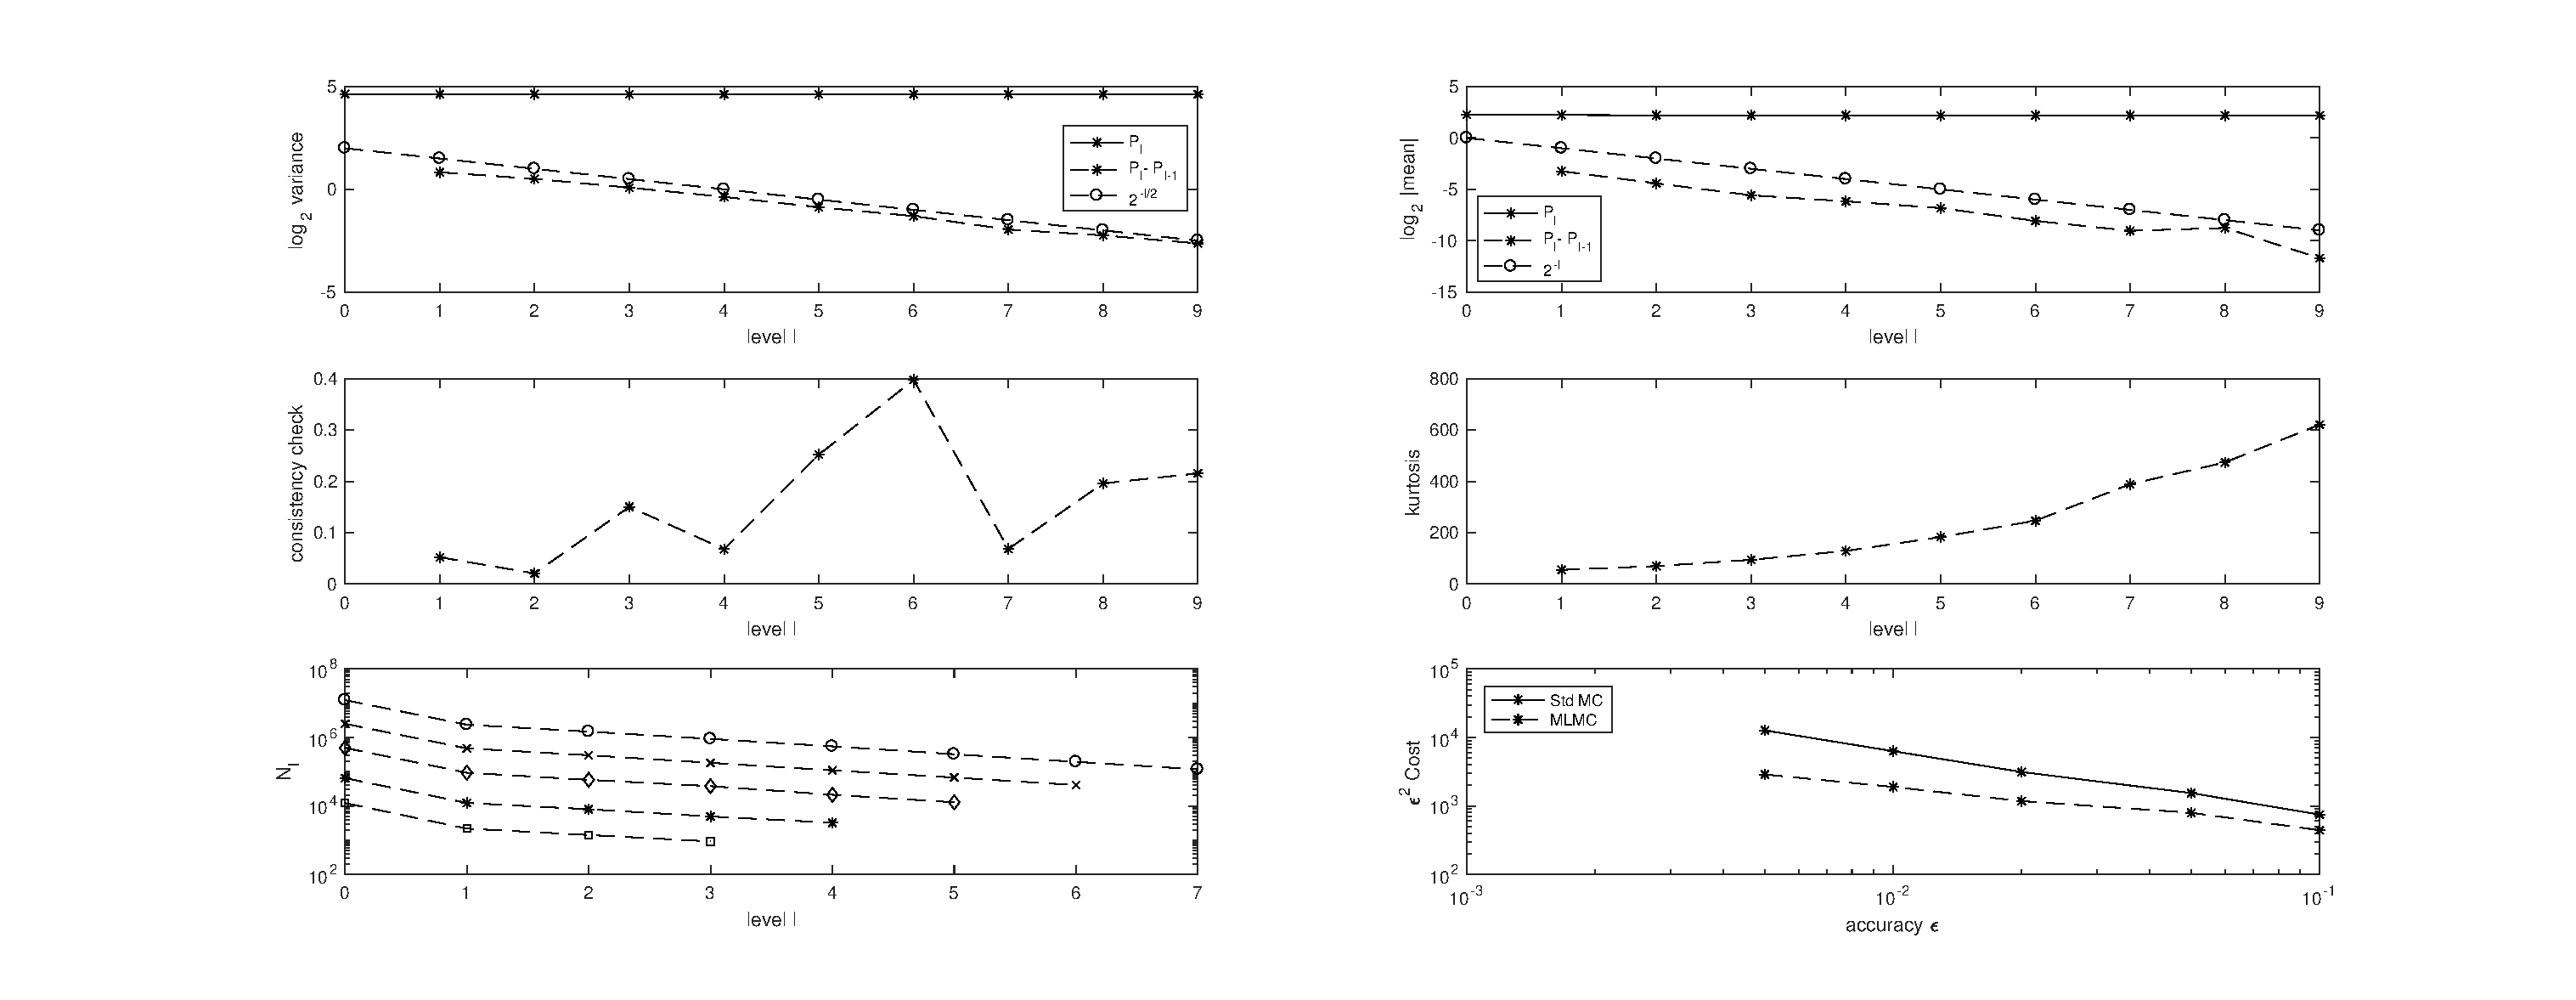
\includegraphics[width=1.2\linewidth]{./figures/MLMC_binary_GBM_opt/euler_digital_without_smoothing_L0_2step}

\caption{Numerical results for a digital call option using the MLMC method coupled with Euler-Maruyama discretisation of the GBM SDE, and without smoothing of the payoff.}
\label{fig:euler_digital_without_smoothing}
\end{figure}

\FloatBarrier
	\begin{figure}[h!]
\centering
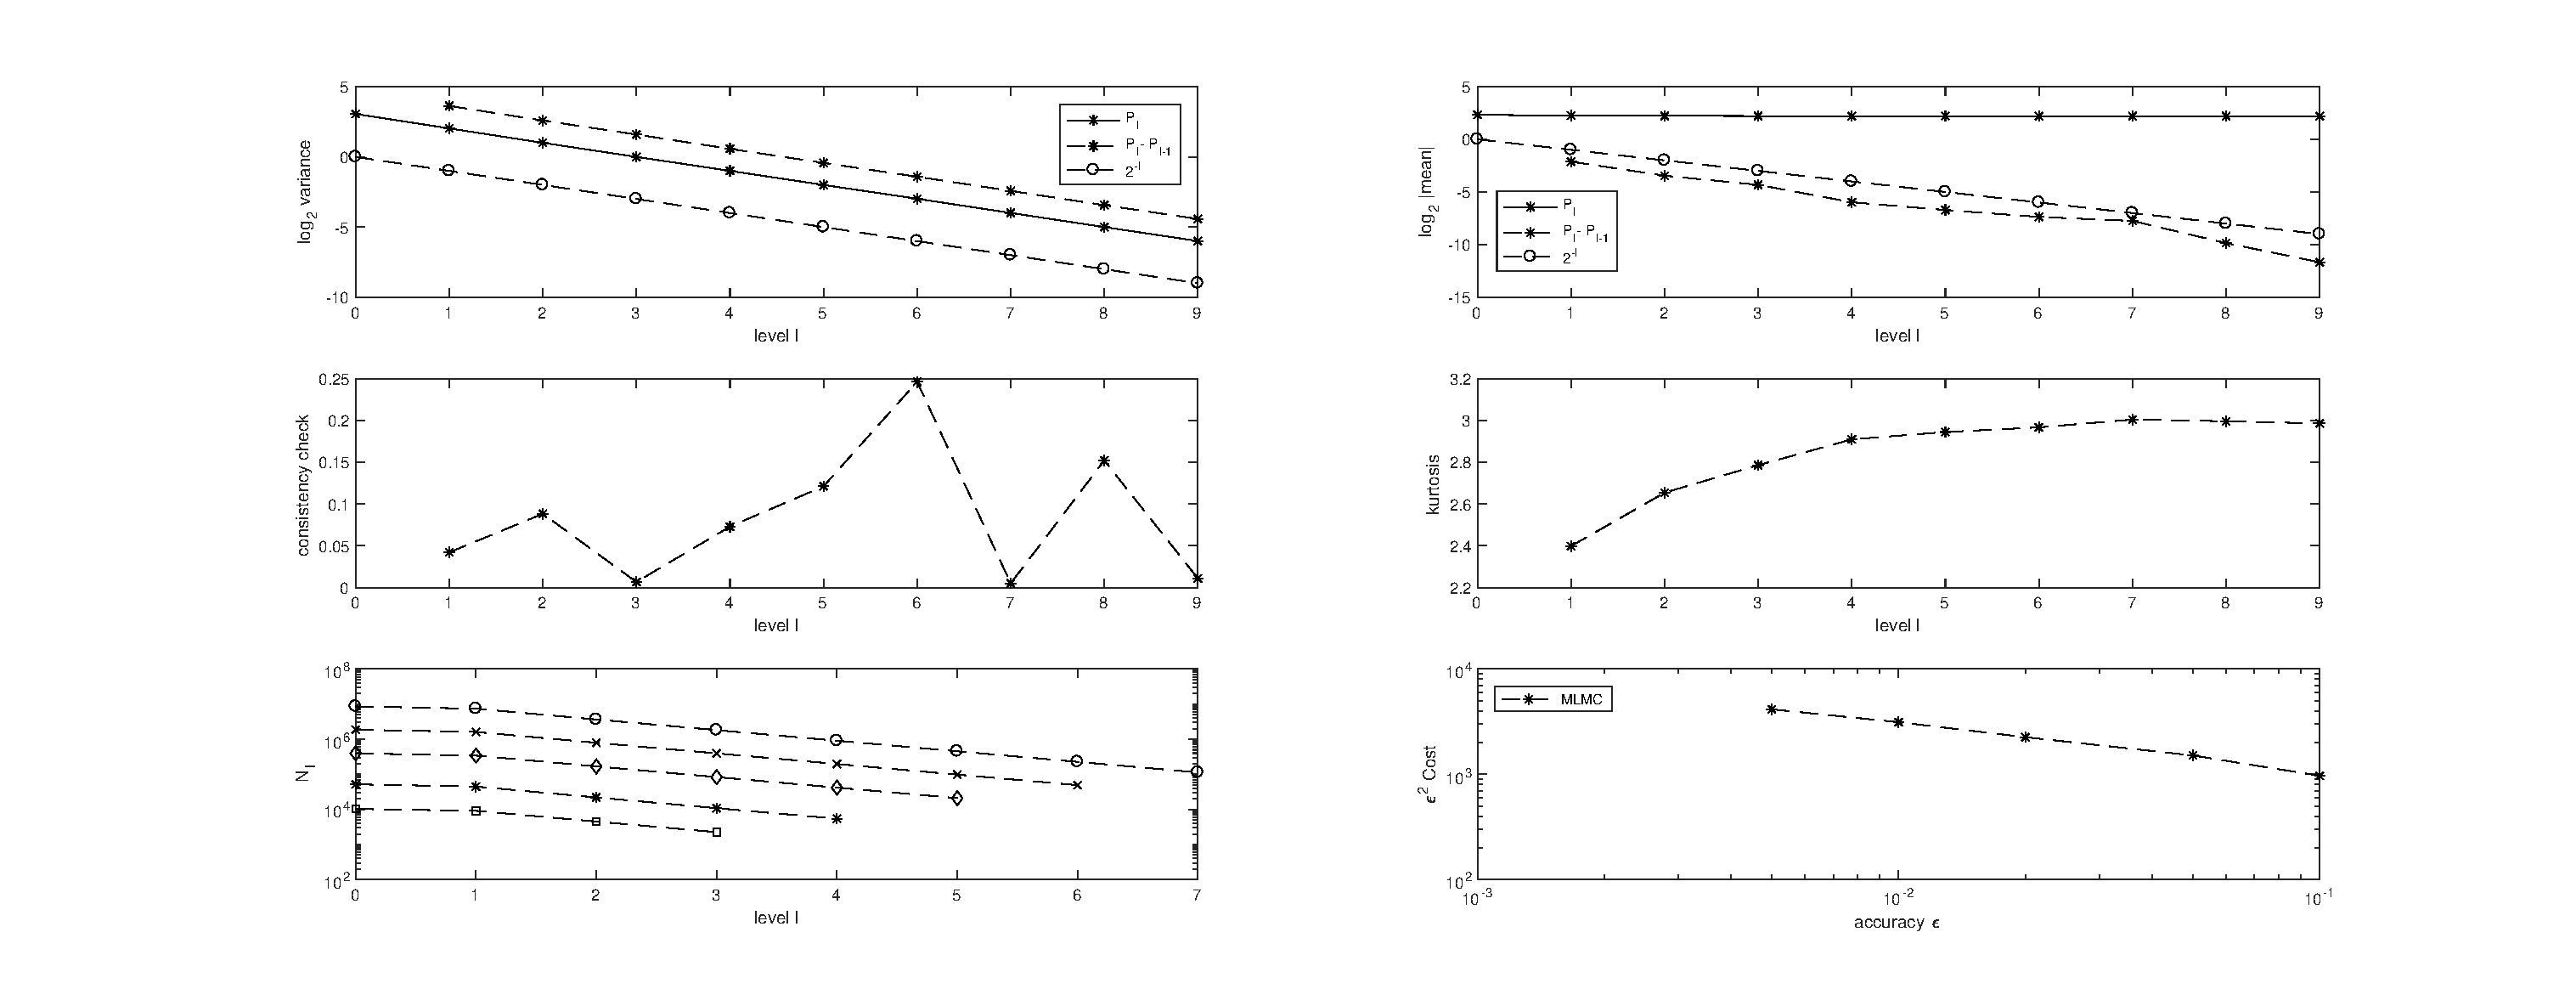
\includegraphics[width=1.2\linewidth]{./figures/MLMC_binary_GBM_opt/digital_option_with_smoothing_L_0_2_steps}

\caption{Numerical results for a digital call option using the MLMC method coupled with Euler-Maruyama discretisation of the GBM SDE, after applying  the numerical smoothing to the payoff. We mention that observing a decaying variance of $P_{\ell}$ here is expected since we used Brownian bridge for path construction, and the QoI depends only on the terminal value of the Brownian bridge which has a variance scaled of order $\Delta t$.}
\label{fig:euler_digital_with_smoothing}
\end{figure}
\FloatBarrier
We emphasize that our approach can be extended in a straightforward manner to any kind of dynamics, since it is based on numerical smoothing based on solving a root finding problem.  In the following Section, we show the advantage of our approach for the Heston model where discretization of the asset price is indeed needed.
\subsubsection{Digital option under the Heston model}\label{sec:Digital option under the Heston model}

Since the asset price in the  Heston model (see \eqref{eq:dynamics Heston})   has similar structure of dynamics compared to the GBM with the difference of the volatility being non constant, we can use  similar idea introduced in Section \ref{sec:The discretized 1D Black-Scholes} and show that
\begin{align}
\expt{g(X)}&=\expt{\mathbf{1}_{X>K}}\nonumber\\
&=\expt{1-\Phi(y^\ast(K))},
\end{align}
where $y^\ast(K)$ is the kink location obtained by solving numerically 
$$X(T; y^\ast(K), \mathbf{z}_{-1})=K,$$
where  $\mathbf{z}$ is $2N-1$ Gaussian random  vector ($N$ is the number of time steps) used for Brownian bridge construction, and $\Phi$ is the cumulative Gaussian distribution function.

As an illustration, we choose the digital option of Heston asset with parameters: $S_0=K=100$, $v_0=0.04$, $\mu=0$,  $\rho=-0.9$, $\kappa=1$, $\xi=0.1$, $\theta=0.0025$, and we compare MLMC results with the original payoff function (without numerical smoothing), given by Figure \ref{fig:euler_digital_Heston_without_smoothing},  and MLMC results after applying our numerical smoothing idea, when using the smooth scheme (see Figure \ref{fig:euler_digital_Heston_with_smoothing_OU}), and the Full truncation scheme (see Figure \ref{fig:euler_digital_Heston_with_smoothing_FT}). From these two Figures we have the following conclusions:
\begin{enumerate}

\item The numerical smoothing has improved the strong rate for  the example under Heston model from $\beta=2/3$ to $\beta=9/10$ for the full truncation scheme resulting in an improvement of the MLMC complexity from  $\Ordo{TOL^{-2.5}}$ to $\Ordo{TOL^{-2}}$ (compare  top left plots in Figures \ref{fig:euler_digital_Heston_without_smoothing}, and Figure \ref{fig:euler_digital_Heston_with_smoothing_FT}).
\item The numerical smoothing has also dropped significantly the kurtosis at the finest level, $\kappa_L$,  by a factor $28$, this is can be seen clearly by comparing the middle right plots in Figures \ref{fig:euler_digital_Heston_without_smoothing}, Figure \ref{fig:euler_digital_Heston_with_smoothing_OU} and Figure \ref{fig:euler_digital_Heston_with_smoothing_FT}. We stress that this is an important improvement, since one needs $\Ordo{\kappa}$ samples  to obtain a reasonable estimate for the variance (see Section \ref{sec:General motivation}).   Note also that although the initial level of MLMC is different for case without smoothing compared to the case we do smoothing, the final levels have the same time mesh that is $\Delta t_{L}=2^{-6}.T$.
\item Improving the strong error rate after using the numerical smoothing, resulted in a slight improvement of the complexity (compare the bottom right plots Figures \ref{fig:euler_digital_Heston_without_smoothing}, Figure \ref{fig:euler_digital_Heston_with_smoothing_OU} and Figure \ref{fig:euler_digital_Heston_with_smoothing_FT}).
\item Finally, observe that we observed slightly better behavior for the case of numerical smoothing using the full truncation scheme (scheme in Section \ref{sec:Discretization of Heston model with a non smooth transformations for the volatility process}) than the smooth scheme when coupled with numerical smoothing  (scheme in Section \ref{sec:Discretization of Heston model with the volatility process Simulated using the sum of  Ornstein-Uhlenbeck (Bessel) processes})  (compare Figures \ref{fig:euler_digital_Heston_with_smoothing_OU} and  \ref{fig:euler_digital_Heston_with_smoothing_FT}).
\end{enumerate}



\FloatBarrier
\begin{figure}[htb]
	\centering % <-- added
	\begin{subfigure}{0.5\textwidth}
		\includegraphics[width=\linewidth]{./figures/MLMC_binary_Heston_opt/without_smoothing/digital_option_set1_L_0_1_steps_L_6_2_N_10_7/digital_option_set1_L_0_1_steps_L_6_2_N_10_7_weak}
		\caption{}
		\label{fig:weak_rate_hest_digital_non_smoothing_FT}
	\end{subfigure}\hfil %% <-- added
	\begin{subfigure}{0.5\textwidth}
		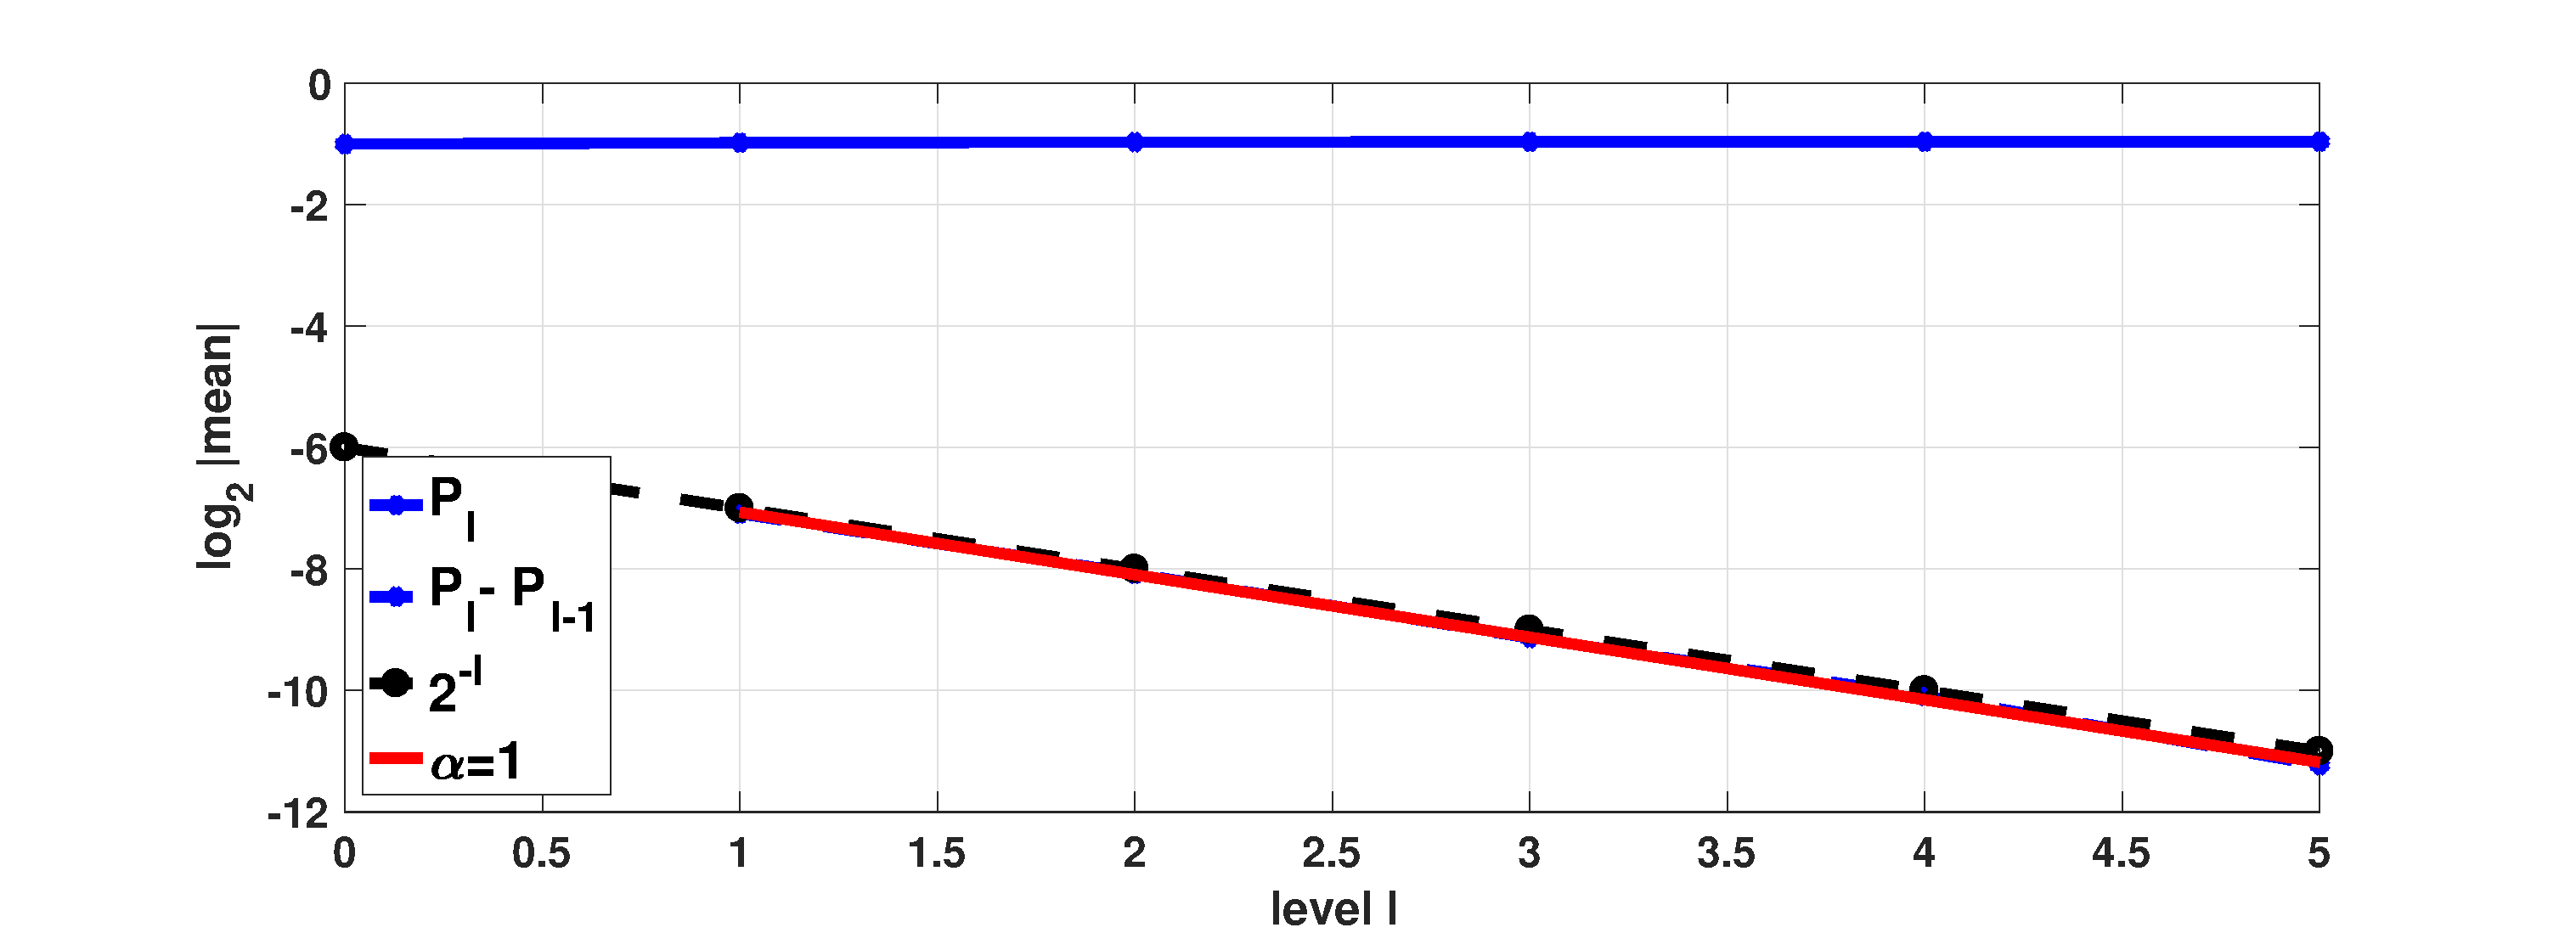
\includegraphics[width=\linewidth]{./figures/MLMC_binary_Heston_opt/with_smoothing/OU/digital_option_set1_L_0_2_steps_L_5_N_10_7_beta_128/digital_option_set1_L_0_2_steps_L_5_N_10_7_weak}
		\caption{}
		\label{fig:weak_rate_hest_digital_smoothing_OU}
	\end{subfigure}\hfil %% <-- added
	\begin{subfigure}{0.5\textwidth}
		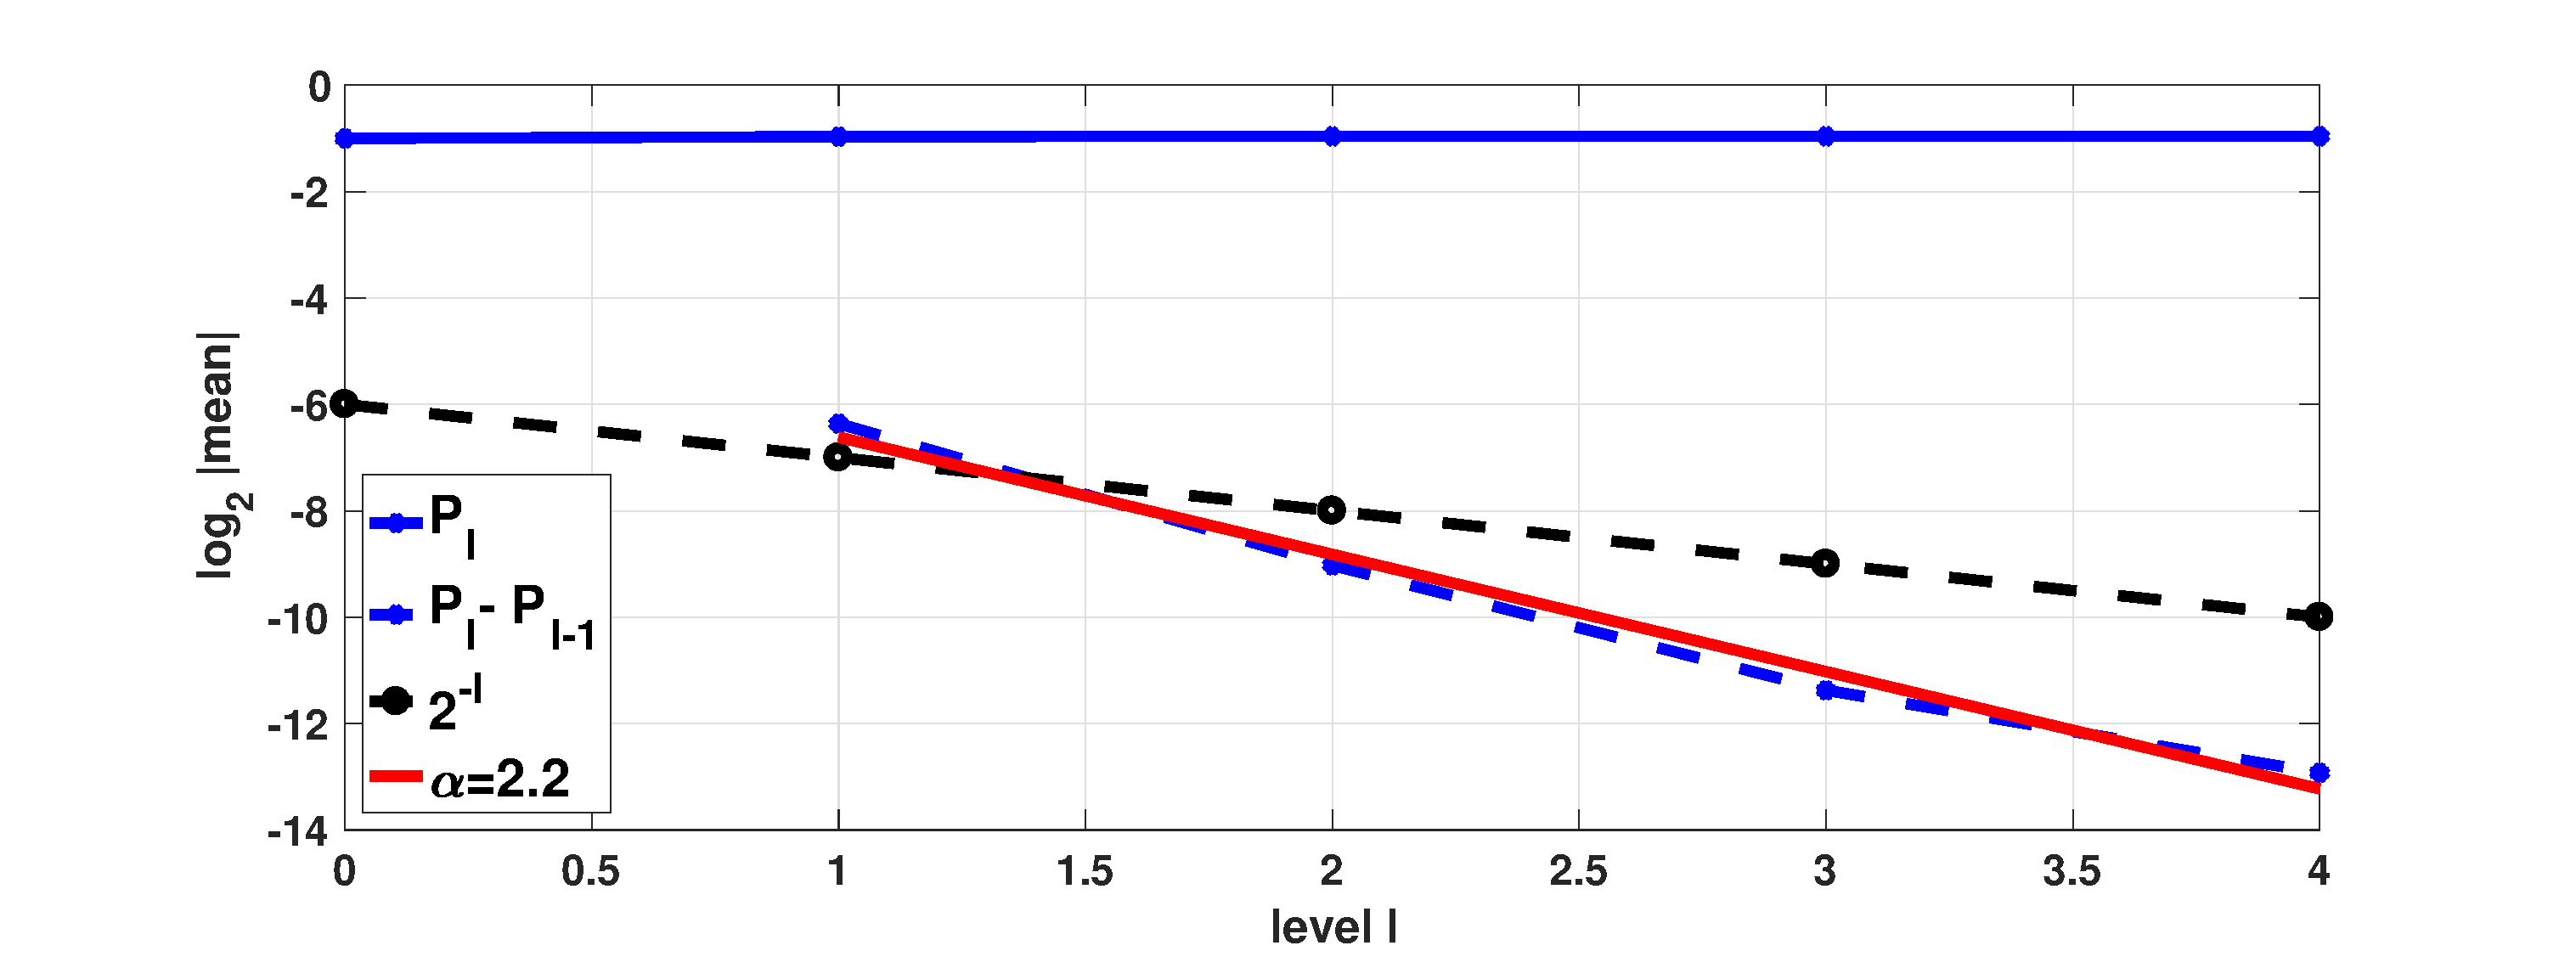
\includegraphics[width=\linewidth]{./figures/MLMC_binary_Heston_opt/with_smoothing/FT/digital_option_set1_L_0_2_steps_L_4_N_10_7_beta_32/digital_option_set1_L_0_2_steps_L_4_N_10_7_weak}
		\caption{}
		\label{fig:weak_rate_hest_digital_smoothing_FT}
	\end{subfigure}
	\caption{Convergence of the weak error,  $\expt{P_{\ell}-P_{\ell-1}}$. a) MLMC without smoothing, b) MLMC with numerical smoothing using the smooth scheme defined in Section \ref{sec:Discretization of Heston model with the volatility process Simulated using the sum of  Ornstein-Uhlenbeck (Bessel) processes}, c) MLMC with numerical smoothing using the full truncation scheme defined in Section \ref{sec:Discretization of Heston model with a non smooth transformations for the volatility process}. Estimation done with $M=10^7$ samples.}
	\label{fig:weak_rate_hest_digital}	
\end{figure}
\FloatBarrier

\begin{figure}[htb]
	\centering % <-- added
	\begin{subfigure}{0.5\textwidth}
		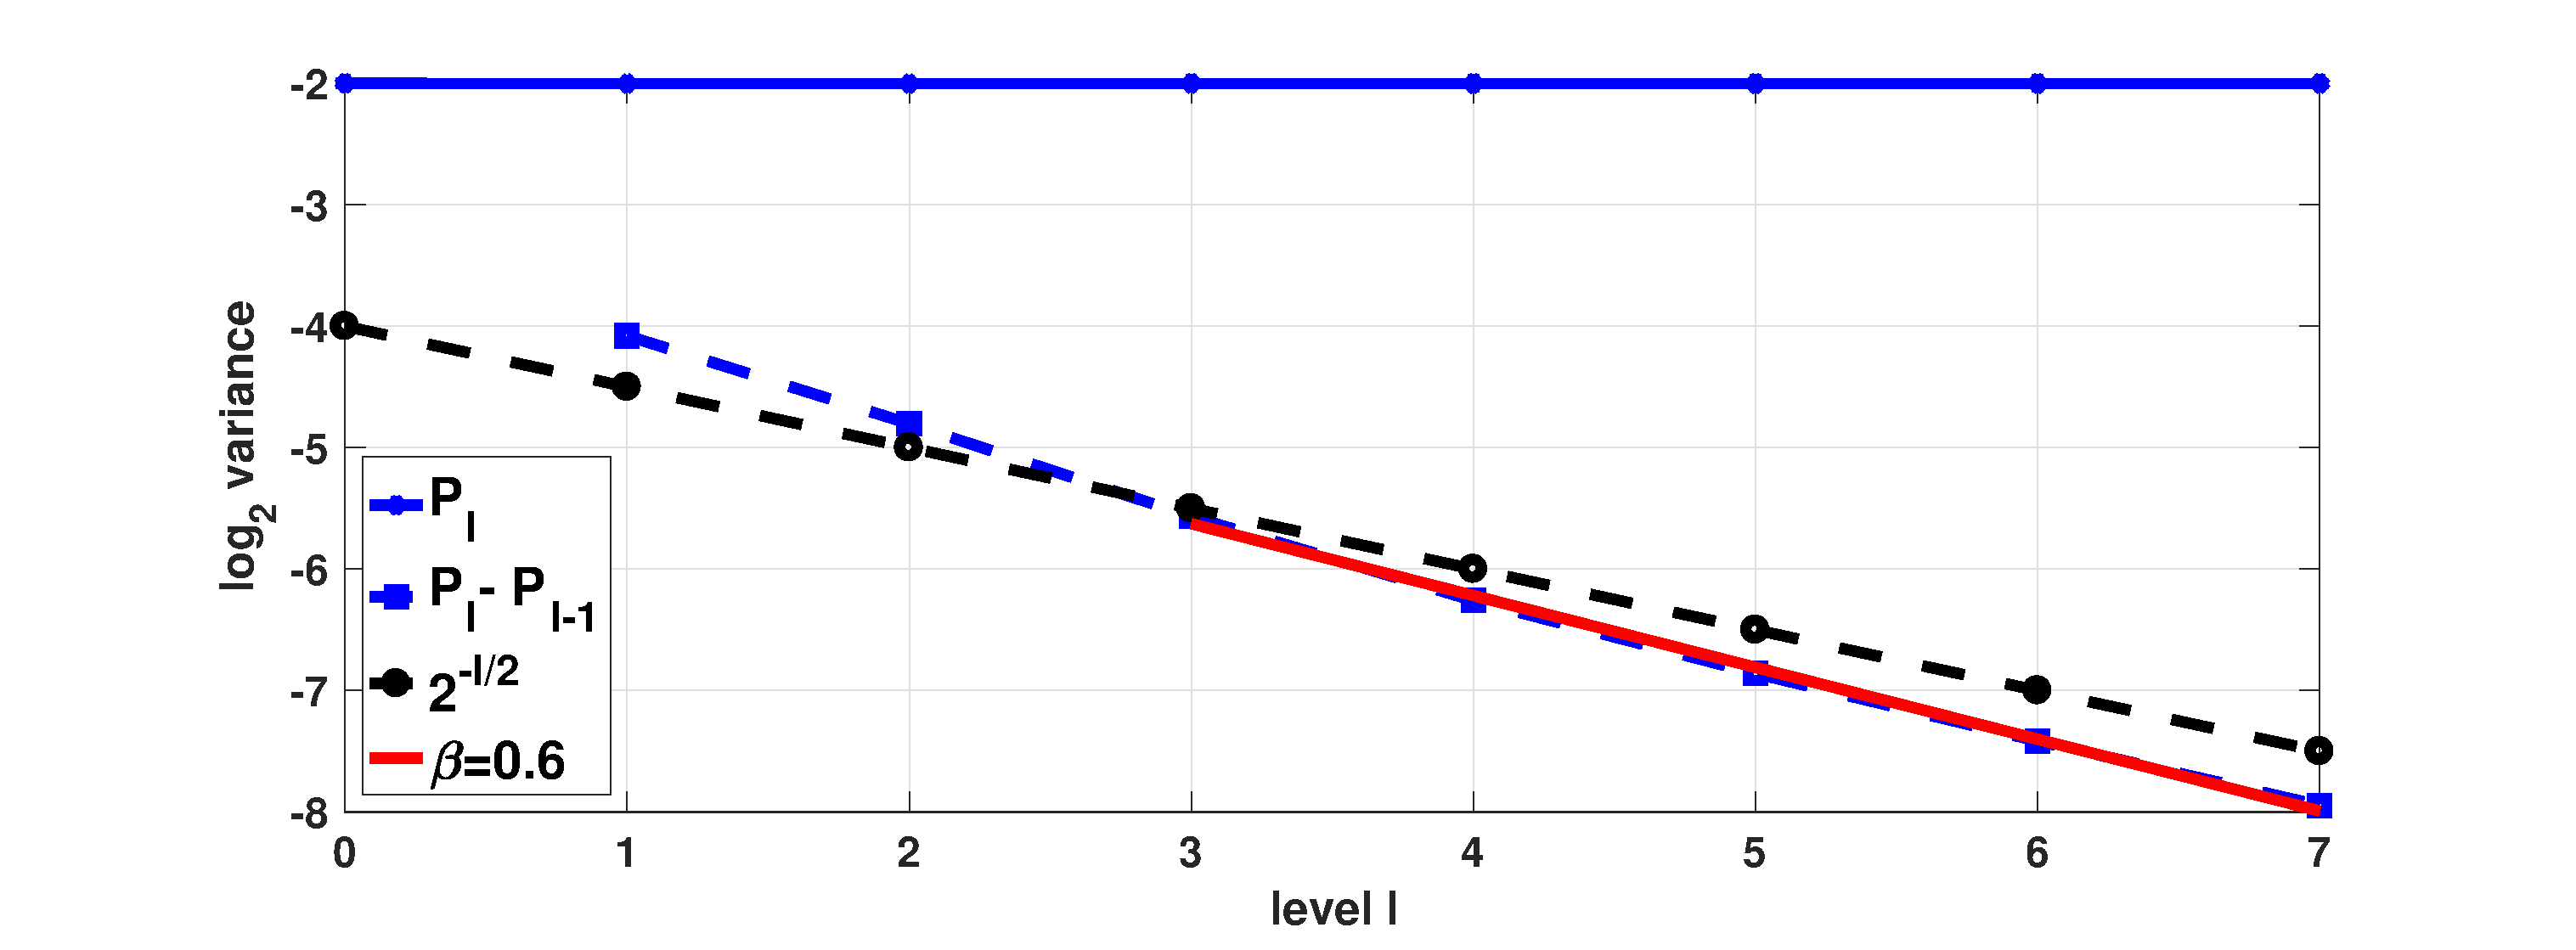
\includegraphics[width=\linewidth]{./figures/MLMC_binary_Heston_opt/without_smoothing/digital_option_set1_L_0_1_steps_L_6_2_N_10_7/digital_option_set1_L_0_1_steps_L_6_2_N_10_7_strong}
		\caption{}
		\label{fig:strong_rate_hest_digital_non_smoothing_FT}
	\end{subfigure}\hfil %% <-- added
	\begin{subfigure}{0.5\textwidth}
		\includegraphics[width=\linewidth]{./figures/MLMC_binary_Heston_opt/with_smoothing/OU/digital_option_set1_L_0_2_steps_L_5_N_10_7_beta_128/digital_option_set1_L_0_2_steps_L_5_N_10_7_strong}
		\caption{}
		\label{fig:strong_rate_hest_digital_smoothing_OU}
	\end{subfigure}\hfil %% <-- added
	\begin{subfigure}{0.5\textwidth}
		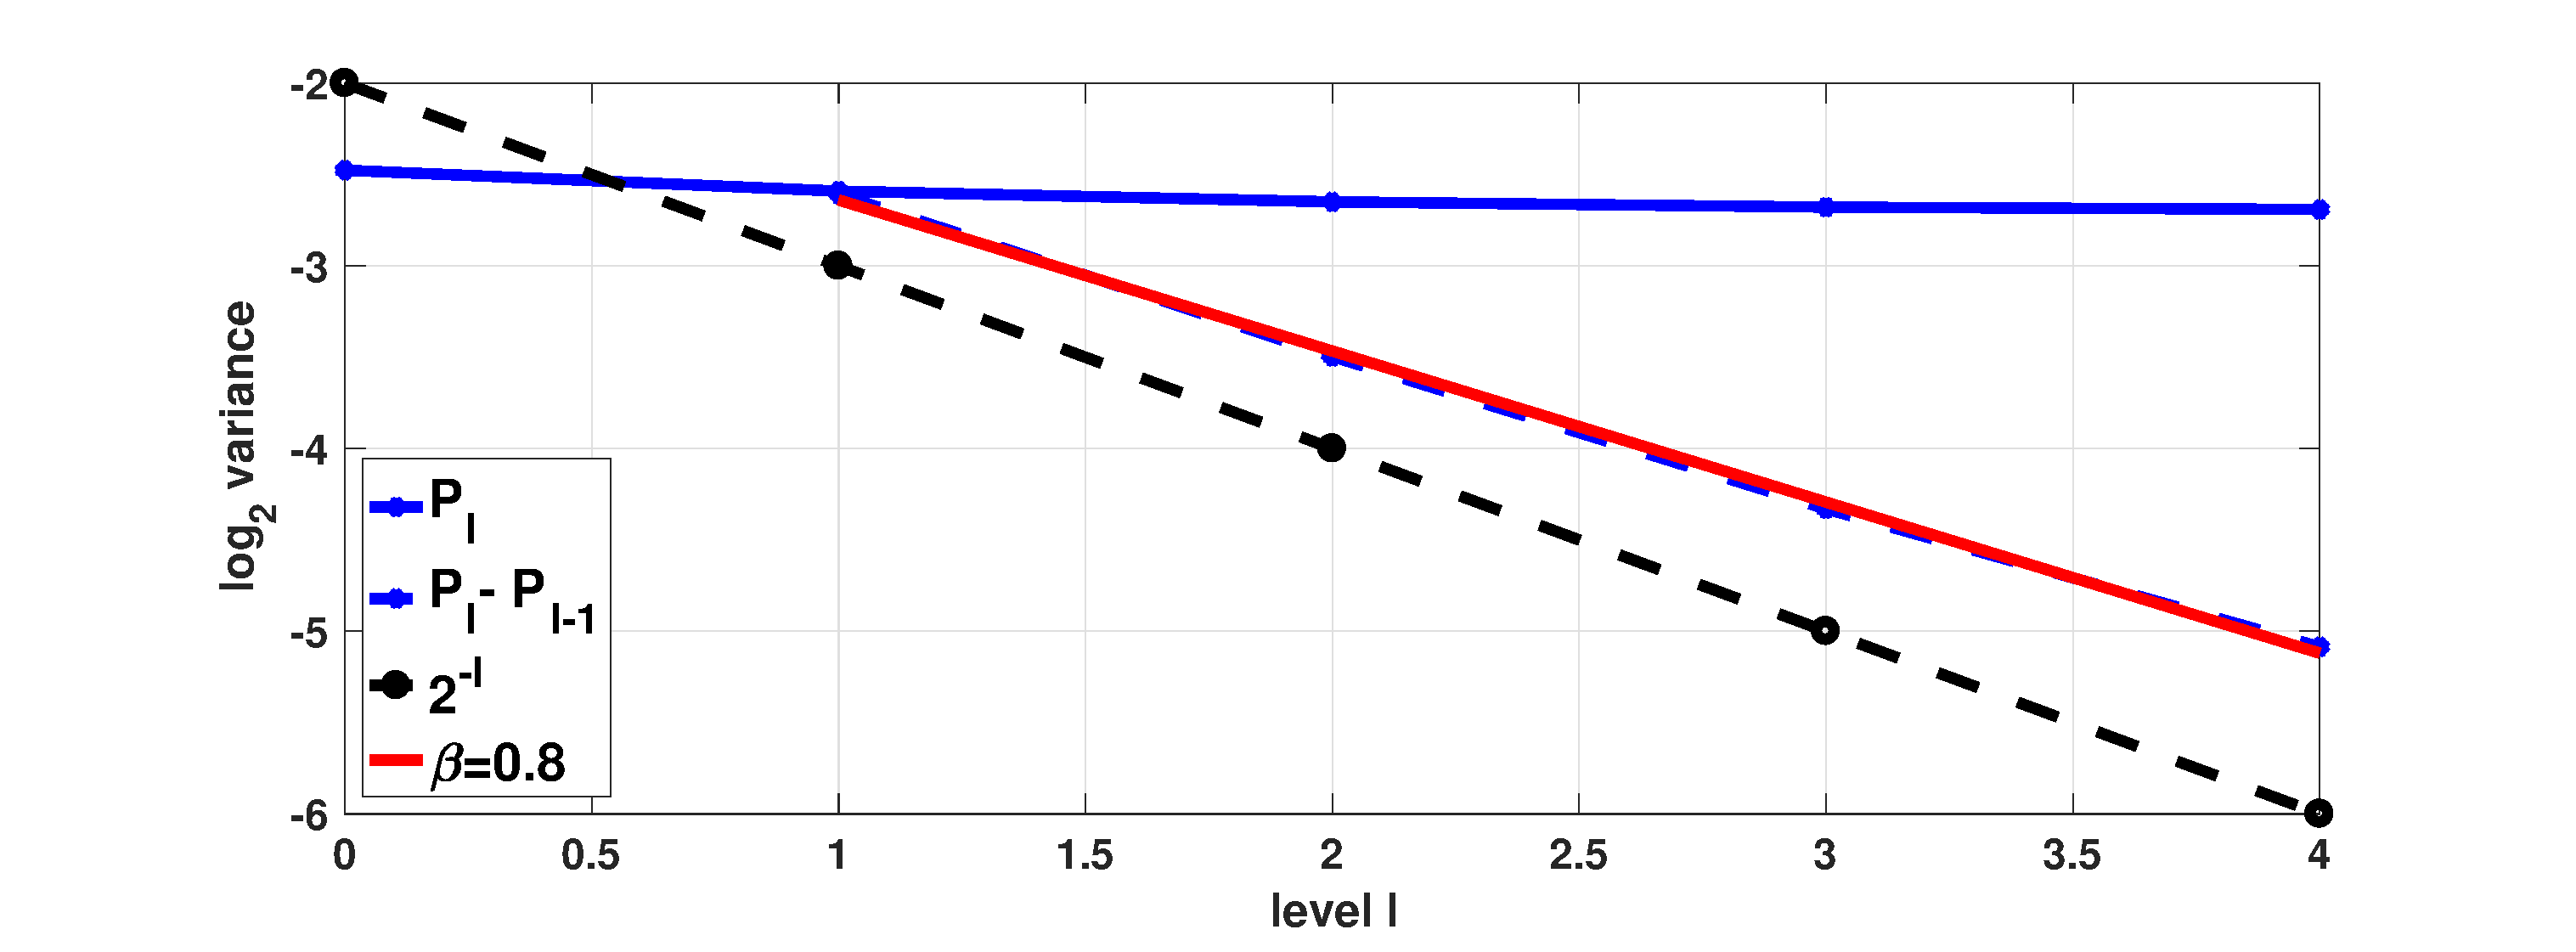
\includegraphics[width=\linewidth]{./figures/MLMC_binary_Heston_opt/with_smoothing/FT/digital_option_set1_L_0_2_steps_L_4_N_10_7_beta_32/digital_option_set1_L_0_2_steps_L_4_N_10_7_strong}
		\caption{}
		\label{fig:strong_rate_hest_digital_smoothing_FT}
	\end{subfigure}
	\caption{Convergence of  the strong error, $\text{Var}\left[P_{\ell}-P_{\ell-1}\right]$. a) MLMC without smoothing, b) MLMC with numerical smoothing using the smooth scheme defined in Section \ref{sec:Discretization of Heston model with the volatility process Simulated using the sum of  Ornstein-Uhlenbeck (Bessel) processes}, c) MLMC with numerical smoothing using the full truncation scheme defined in Section \ref{sec:Discretization of Heston model with a non smooth transformations for the volatility process}.  Estimation done with $M=10^7$ samples.}
	\label{fig:strong_rate_hest_digital}	
\end{figure}
\FloatBarrier

%
%\begin{figure}[htb]
%	\centering % <-- added
%	\begin{subfigure}{0.4\textwidth}
%		\includegraphics[width=\linewidth]{./figures/MLMC_binary_Heston_opt/without_smoothing/digital_option_set1_L_0_1_steps_L_6_2_N_10_7/digital_option_set1_L_0_1_steps_L_6_2_N_10_7_complexity}
%		\caption{}
%		\label{fig:complex_rate_hest_digital_non_smoothing_FT}
%	\end{subfigure}\hfil %% <-- added
%	\begin{subfigure}{0.4\textwidth}
%		\includegraphics[width=\linewidth]{./figures/MLMC_binary_Heston_opt/with_smoothing/OU/digital_option_set1_L_0_2_steps_L_5_N_10_7_beta_128/digital_option_set1_L_0_2_steps_L_5_N_10_7_complexity}
%		\caption{}
%		\label{fig:complex_rate_hest_digital_smoothing_OU}
%	\end{subfigure}\hfil %% <-- added
%	\begin{subfigure}{0.4\textwidth}
%		\includegraphics[width=\linewidth]{./figures/MLMC_binary_Heston_opt/with_smoothing/FT/digital_option_set1_L_0_2_steps_L_5_N_10_7_beta_128/digital_option_set1_L_0_2_steps_L_5_N_10_7_complexity}
%		\caption{}
%		\label{fig:strong_rate_hest_digital_smoothing_FT}
%	\end{subfigure}
%	\caption{}
%	\label{fig:complex_rate_hest_digital}	
%\end{figure}
%\FloatBarrier

\begin{figure}[htb]
	\centering % <-- added
	\begin{subfigure}{0.5\textwidth}
		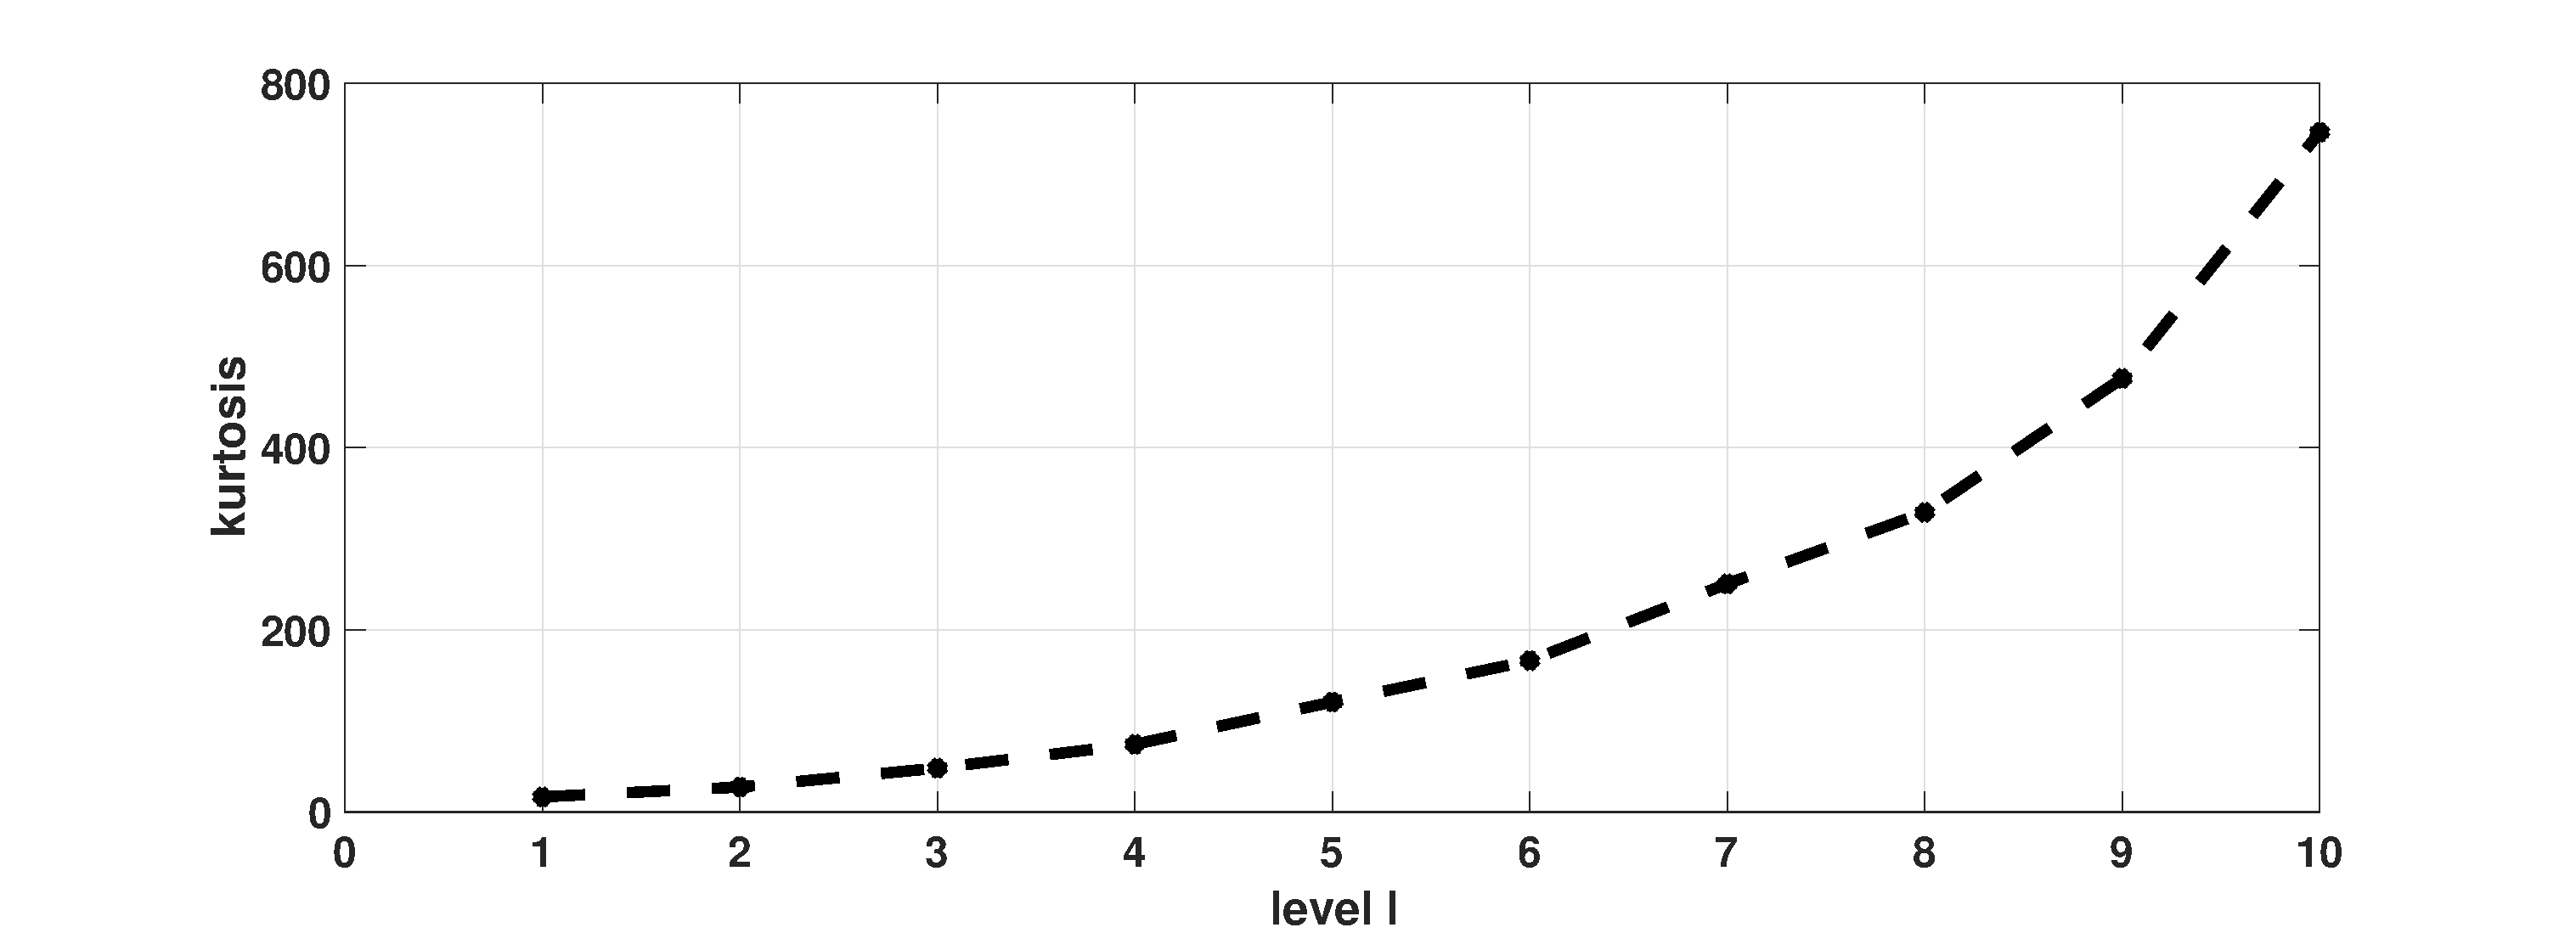
\includegraphics[width=\linewidth]{./figures/MLMC_binary_Heston_opt/without_smoothing/kurtosis_L_0_1_step}
		\caption{}
		\label{fig:kurt_hest_digital_non_smoothing_FT}
	\end{subfigure}\hfil %% <-- added
	\begin{subfigure}{0.5\textwidth}
		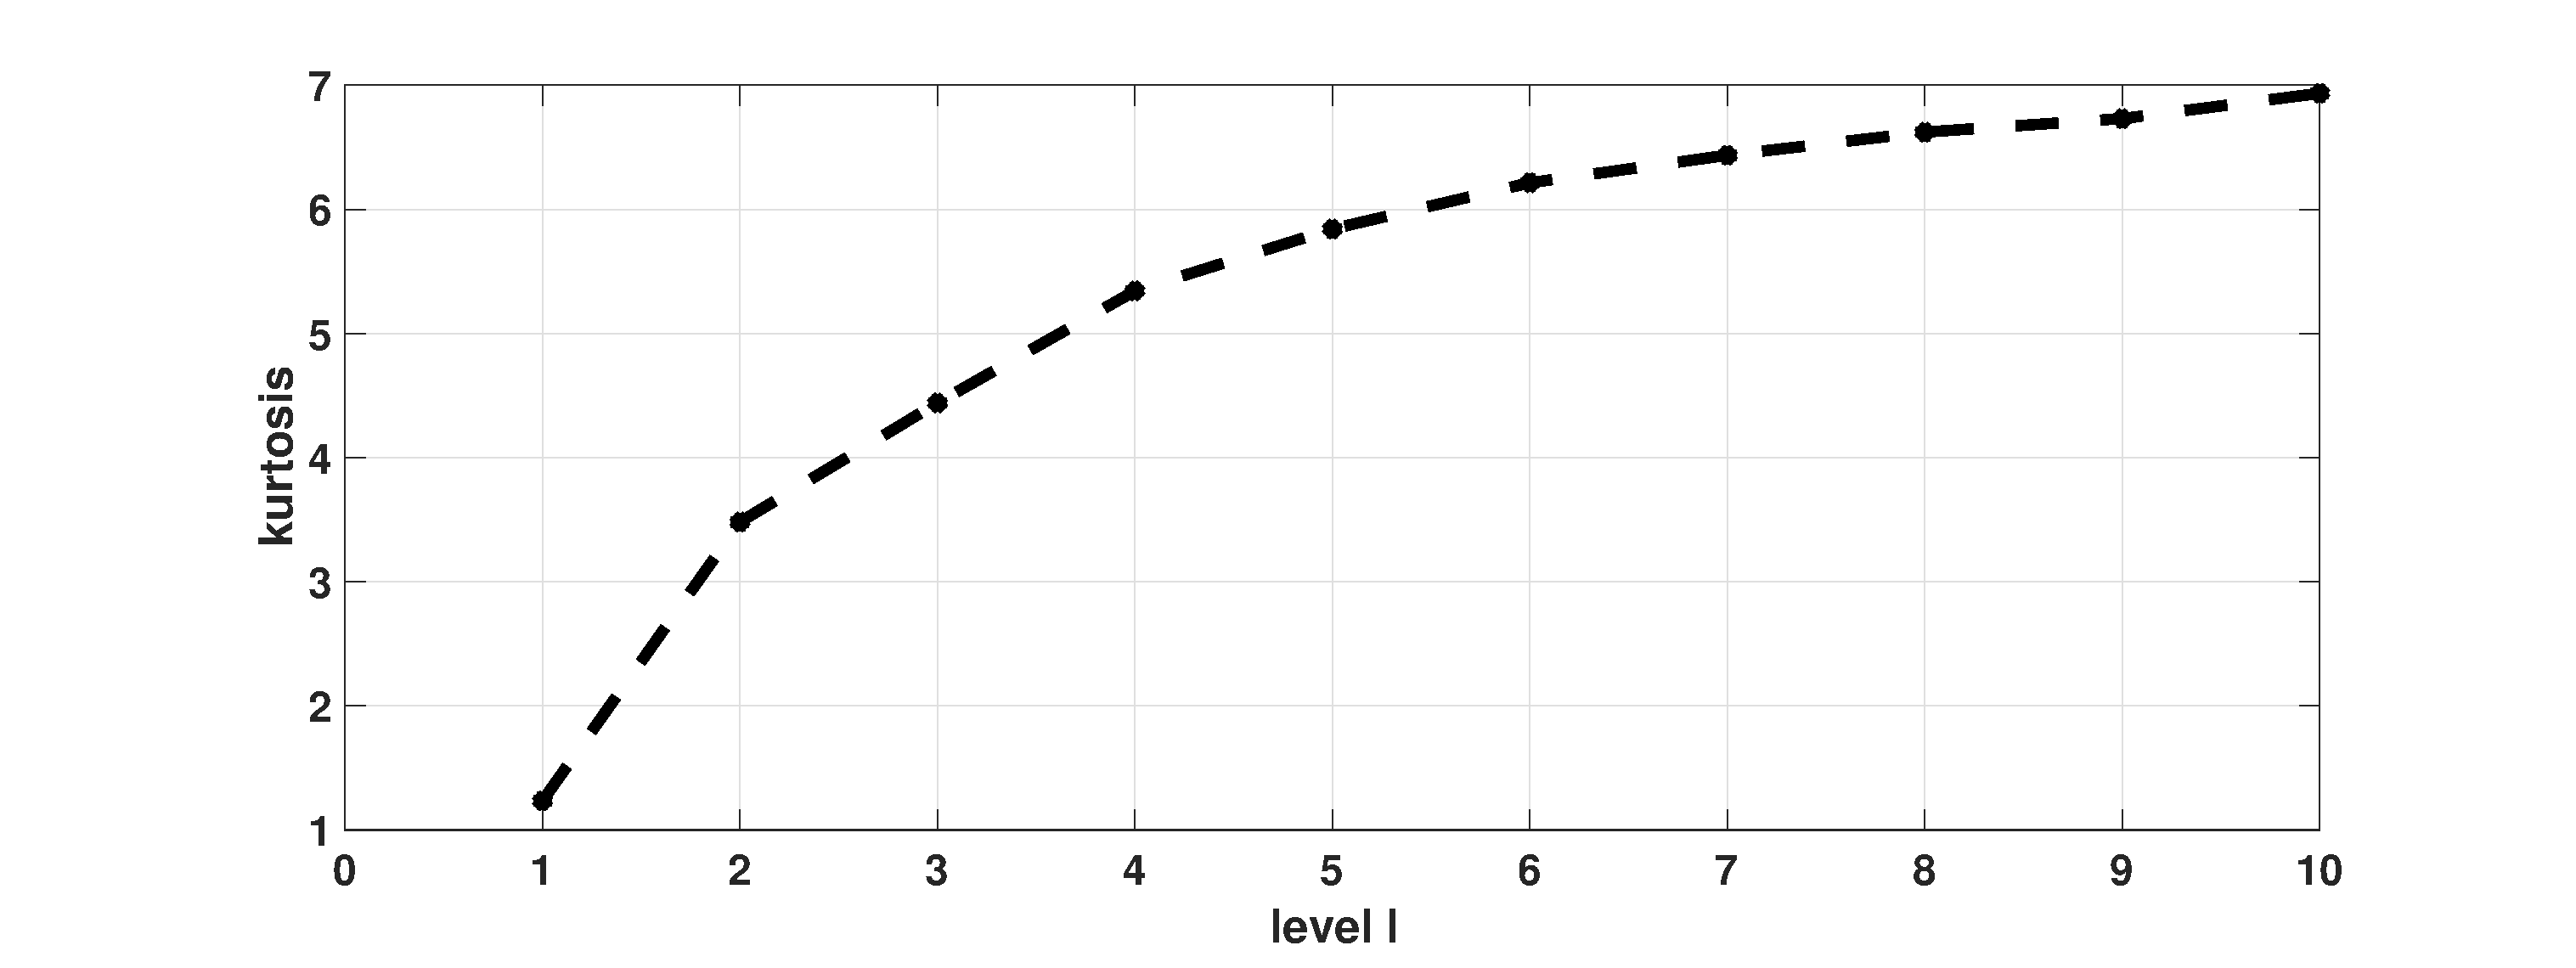
\includegraphics[width=\linewidth]{./figures/MLMC_binary_Heston_opt/with_smoothing/kurtosis}
		\caption{}
		\label{fig:kurt_hest_digital_smoothing}
	\end{subfigure}\hfil %% <-- added
	\caption{Comparison of the kurtosis $\kappa_{\ell}$, defined in \eqref{eq:Kurtosis} between a) MLMC without smoothing and b) MLMC with numerical smoothing. We can see that the numerical smoothing has dropped significantly the kurtosis at the finest level $L=10$  by a factor  of about $107$.  Estimation done with $M=10^7$ samples.}
	\label{fig:kurt_hest_digital}	
\end{figure}
\FloatBarrier

	\begin{figure}[h!]
\centering
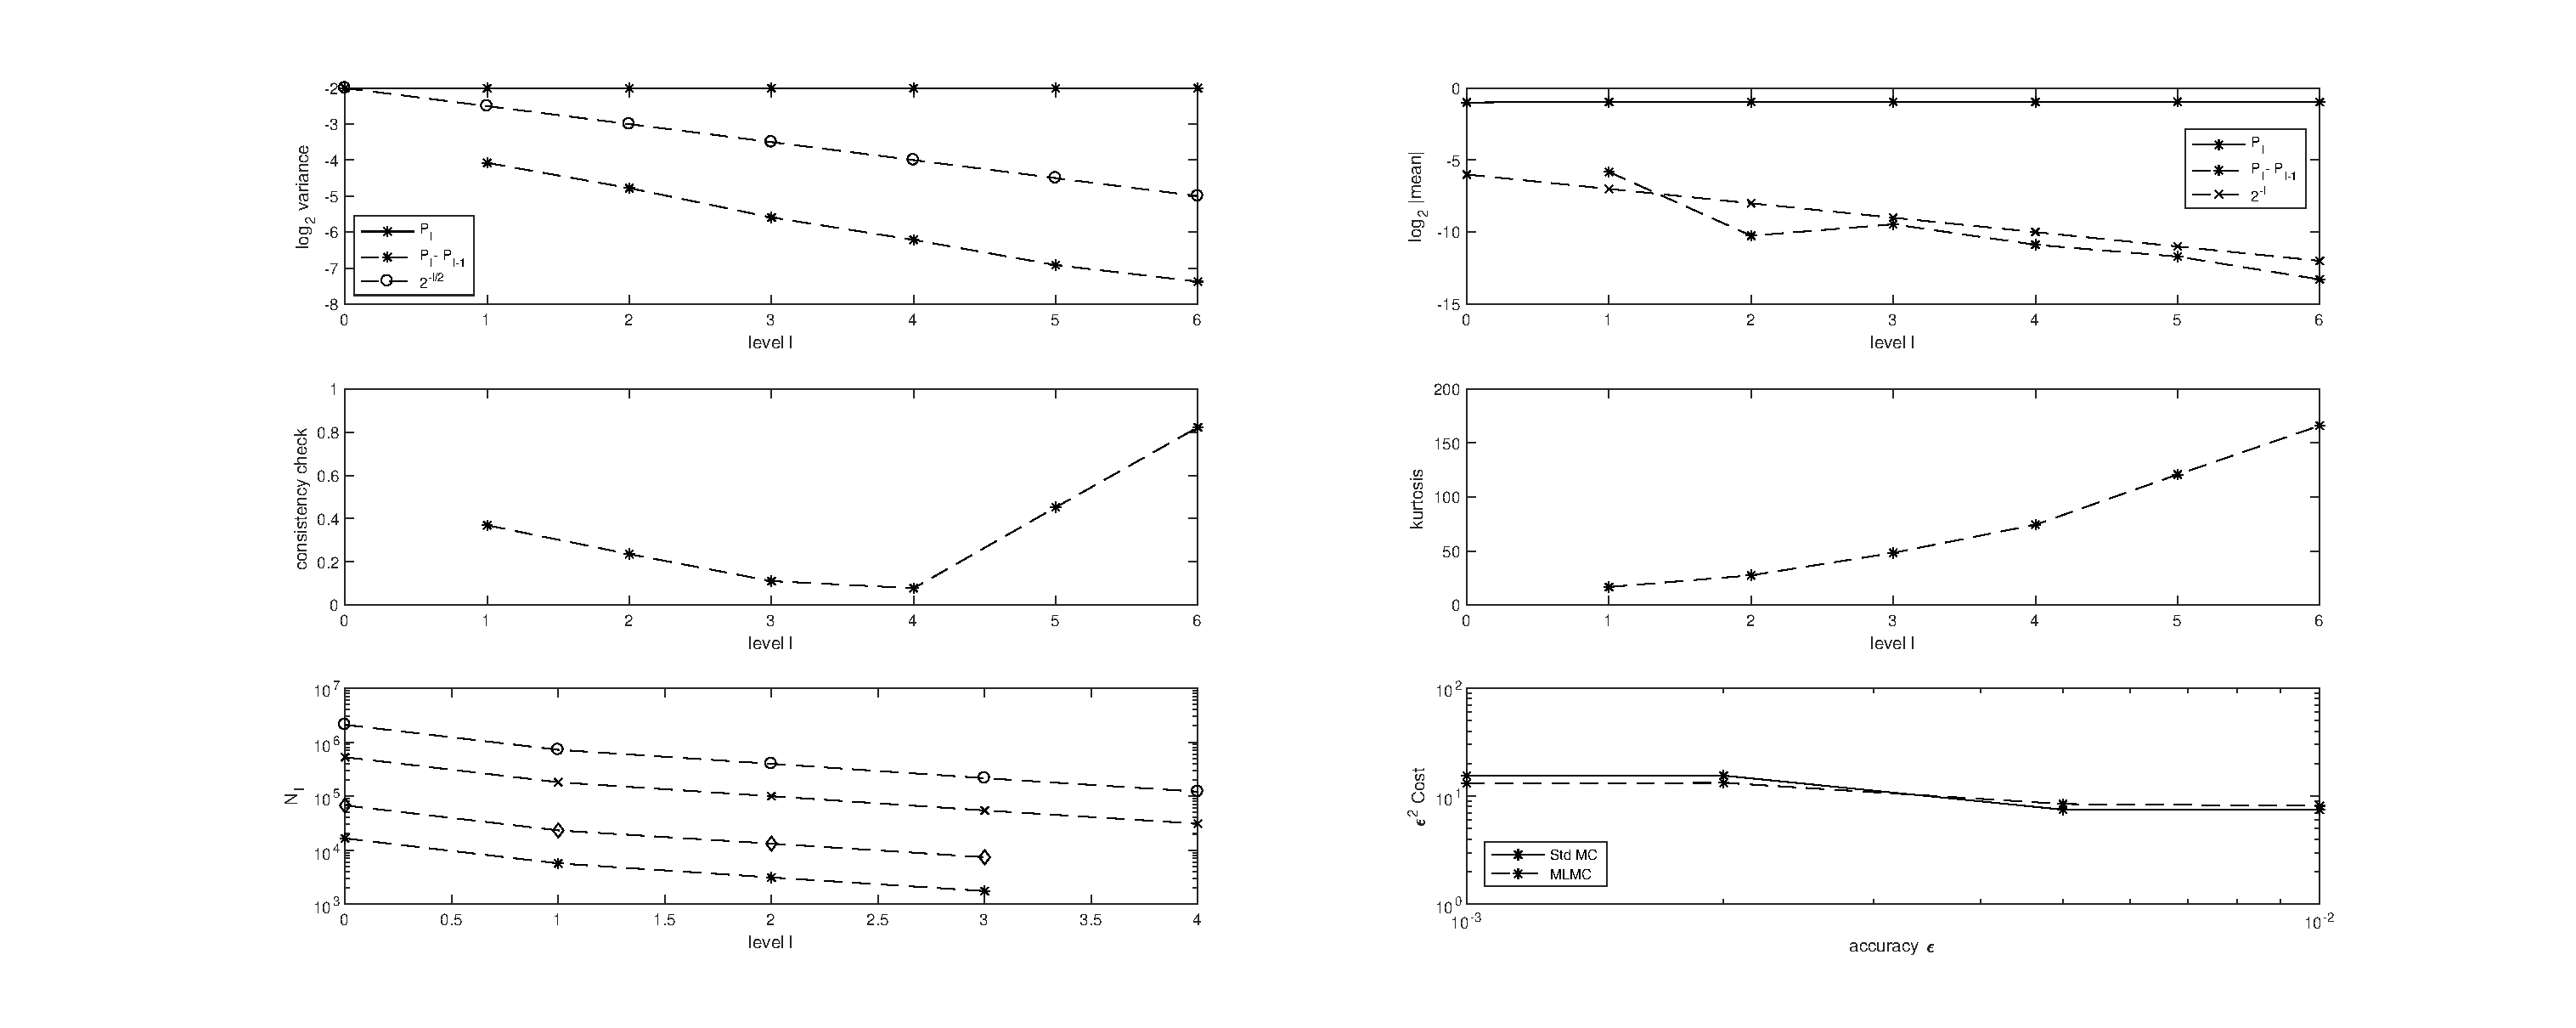
\includegraphics[width=1.2\linewidth]{./figures/MLMC_binary_Heston_opt/without_smoothing/digital_option_set1_L_0_1_steps_L_6}

\caption{Numerical results for a digital call option under the Heston model using the MLMC method coupled with  the Full truncation scheme in Section \ref{sec:Discretization of Heston model with a non smooth transformations for the volatility process}, and without smoothing of the payoff.}
\label{fig:euler_digital_Heston_without_smoothing}
\end{figure}



\FloatBarrier
	\begin{figure}[h!]
\centering
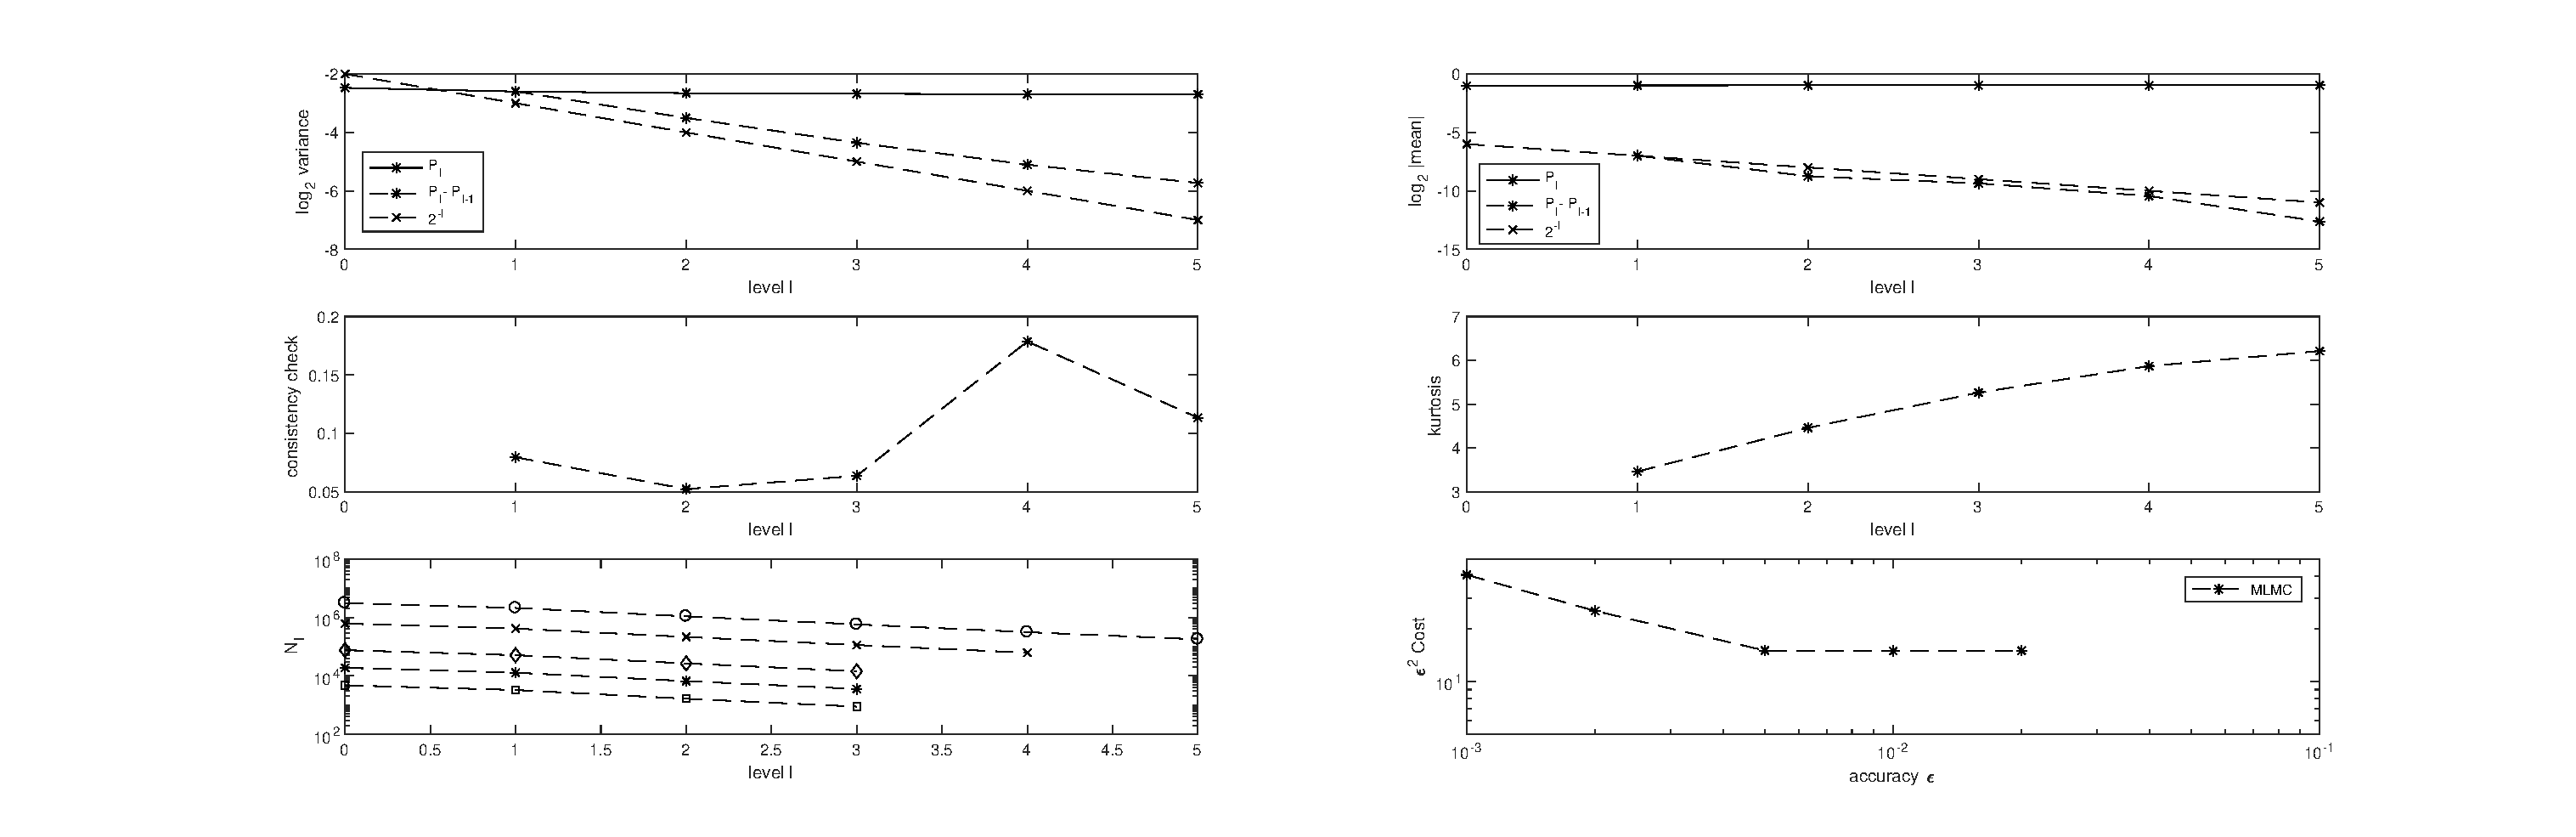
\includegraphics[width=1.2\linewidth]{./figures/MLMC_binary_Heston_opt/with_smoothing/OU/digital_option_set1_L_0_2_steps_L_6}

\caption{Numerical results for a digital call option under the Heston model using the MLMC method coupled with  the smooth   scheme in Section \ref{sec:Discretization of Heston model with the volatility process Simulated using the sum of  Ornstein-Uhlenbeck (Bessel) processes}, and with smoothing of the payoff.}
\label{fig:euler_digital_Heston_with_smoothing_OU}
\end{figure}
\FloatBarrier
	\begin{figure}[h!]
\centering
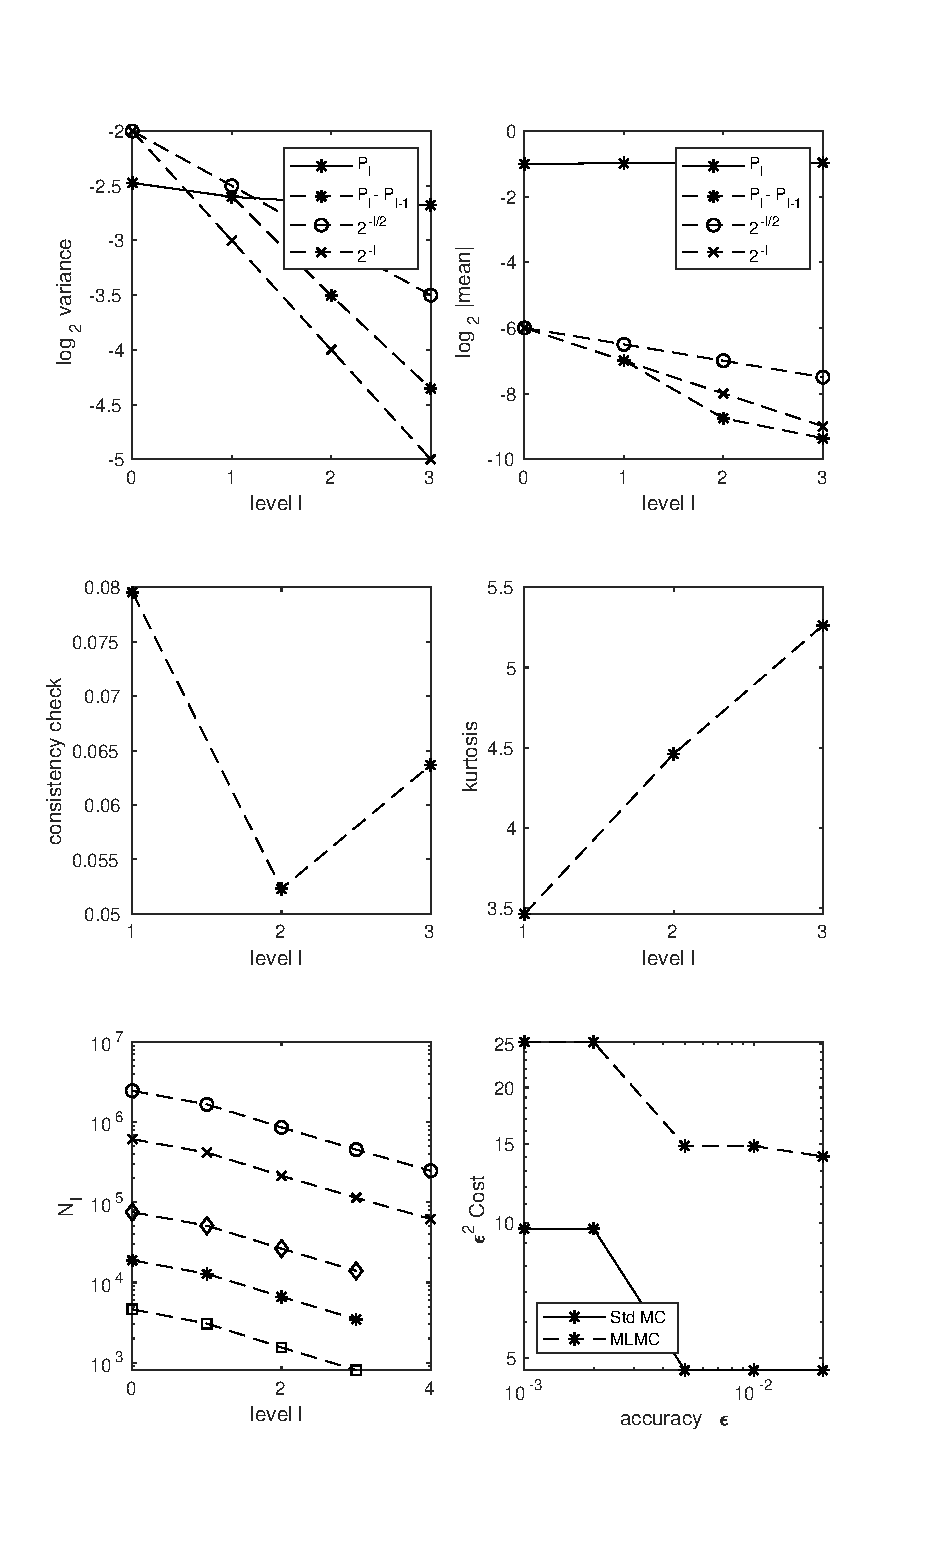
\includegraphics[width=1.2\linewidth]{./figures/MLMC_binary_Heston_opt/with_smoothing/FT/digital_option_set1_L_0_2_steps_L_4}

\caption{Numerical results for a digital call option under the Heston model using the MLMC method coupled with   the Full truncation scheme in Section \ref{sec:Discretization of Heston model with a non smooth transformations for the volatility process}, and with smoothing of the payoff.}
\label{fig:euler_digital_Heston_with_smoothing_FT}
\end{figure}
\FloatBarrier


\begin{remark}
Although we just illustrated the benefit of our approach when coupled with MLMC for computing the digital option price under the GBM (Section \ref{sec:Digital options under the GBM model}) and Heston dynamics (Section \ref{sec:Digital option under the Heston model}), we emphasize that it can be easily extended to any kind of model dynamics and  to any low regular observable, $g$. For instance, this idea can be applied for approximating distribution functions involving the indicator function as the observable $g$. Finally, in all these possible extensions, we expect similar gains to be observed compared to the case of using MLMC without smoothing.
\end{remark}

\subsection{MLMC for approximating densities and Greeks}\label{sec: MLMC for approximating densities and greeks}
In this section, we motivate the idea of coupling the numerical smoothing  with MLMC method to compute density functions and Greeks for non smooth payoff functions. We remind that MLMC without any smoothing  will fail due to the infinite variance caused by the singularity of  the delta function. The aim in this case is to approximate the density, $\rho_{X}(u)$, for a given stochastic process $X$, at point $u$, and which is given by 
\begin{align}
\rho_{X}(u)=\expt{\delta(X-u)},
\end{align}
where $\delta$ is the Dirac delta function.


In Table \ref{table:Summary of our numerical results density.}, we summarize the obtained results for estimating the density, using MLMC coupled with numerical smoothing, under GBM and Heston dynamics. 
\FloatBarrier

\begin{table}[!h]
	\centering
	\begin{small}
	\begin{tabular}{l*{4}{c}r}
	\toprule[1.5pt]
		Method      &   Kurtosis & $\alpha$   &  $\beta$  &  $\gamma$   & Complexity \\
		\hline
			GBM $+$ numerical smoothing & $3.5$ & $1$  &  $1.2$&  $1$&  $TOL^{-2}$\\	
              \hline 
           Heston $+$ numerical smoothing  using smooth scheme & $5$ & $1$  &  $1/2$ & $1$ &  $TOL^{-2.5}$\\	
               \hline
            Heston $+$ numerical smoothing  the full truncation scheme & $6$ & $1$  &  $1/2$&  $1$ &  $TOL^{-2.5}$\\	
		\bottomrule[1.25pt]
	\end{tabular}
\end{small}
	\caption{Summary of the MLMC numerical results observed for  computing the density of asset price under GBM and   Heston models. $\kappa_{L}$ is the kurtosis at the finest levels of MLMC with $\Delta t_{L}=T.2^{-8}$, $(\alpha,\beta,\gamma)$ are weak, strong and work rates respectively. $TOL$ is the user selected  MLMC  tolerance. These results correspond to Figures \ref{fig:euler_density_MLMC_with_smoothing}, \ref{fig:Heston_density_MLMC_with_smoothing_OU} and \ref{fig:Heston_density_MLMC_with_smoothing_FT}.}
	\label{table:Summary of our numerical results density.}
\end{table}
\FloatBarrier

\subsubsection{Approximating density under the GBM model}\label{sec:Approximating density under the GBM model}

We can show that 
\begin{align}
\rho_{X}(u)&=\expt{\delta(X-y)}\nonumber\\
&=\exp\left(-(y^\ast(u))^2/2\right) \frac{d y^\ast}{dx}(u),
\end{align}
where $y^\ast(K)$ is the kink location obtained by solving numerically 
$$X(T; y^\ast(K), \mathbf{z}_{-1})=K,$$
where  $\mathbf{z}$ is $N-1$ Gaussian random  vector ($N$ is the number of time steps) used for Brownian bridge construction.

As an illustration, we choose to compute the density $\rho_{X}$  such that $X$ is a GBM with parameters: $S_0=K=1$, $T=1$, $r=0$, and $\sigma=0.2$. In this case, as a reference solution,  we know that $X(T)$ is lognormally distributed with parameters $r-\sigma^2$ and $\sigma^2$. In Figure \ref{fig:euler_density_MLMC_with_smoothing}, we show the numerical results  for computing the $\rho_{X}$ at $u=1$, using  MLMC coupled with the numerical smoothing idea. From Figure \ref{fig:euler_density_MLMC_with_smoothing}, we can check that we obtain a strong convergence rate of order $3/2$(see  top left plot in Figure \ref{fig:euler_density_MLMC_with_smoothing}), which results in a complexity of the MLMC estimator to be of order $TOL^{-2}$, where $TOL$ is a prescribed tolerance.



\begin{figure}[htb]
	\centering % <-- added
	\begin{subfigure}{0.5\textwidth}
		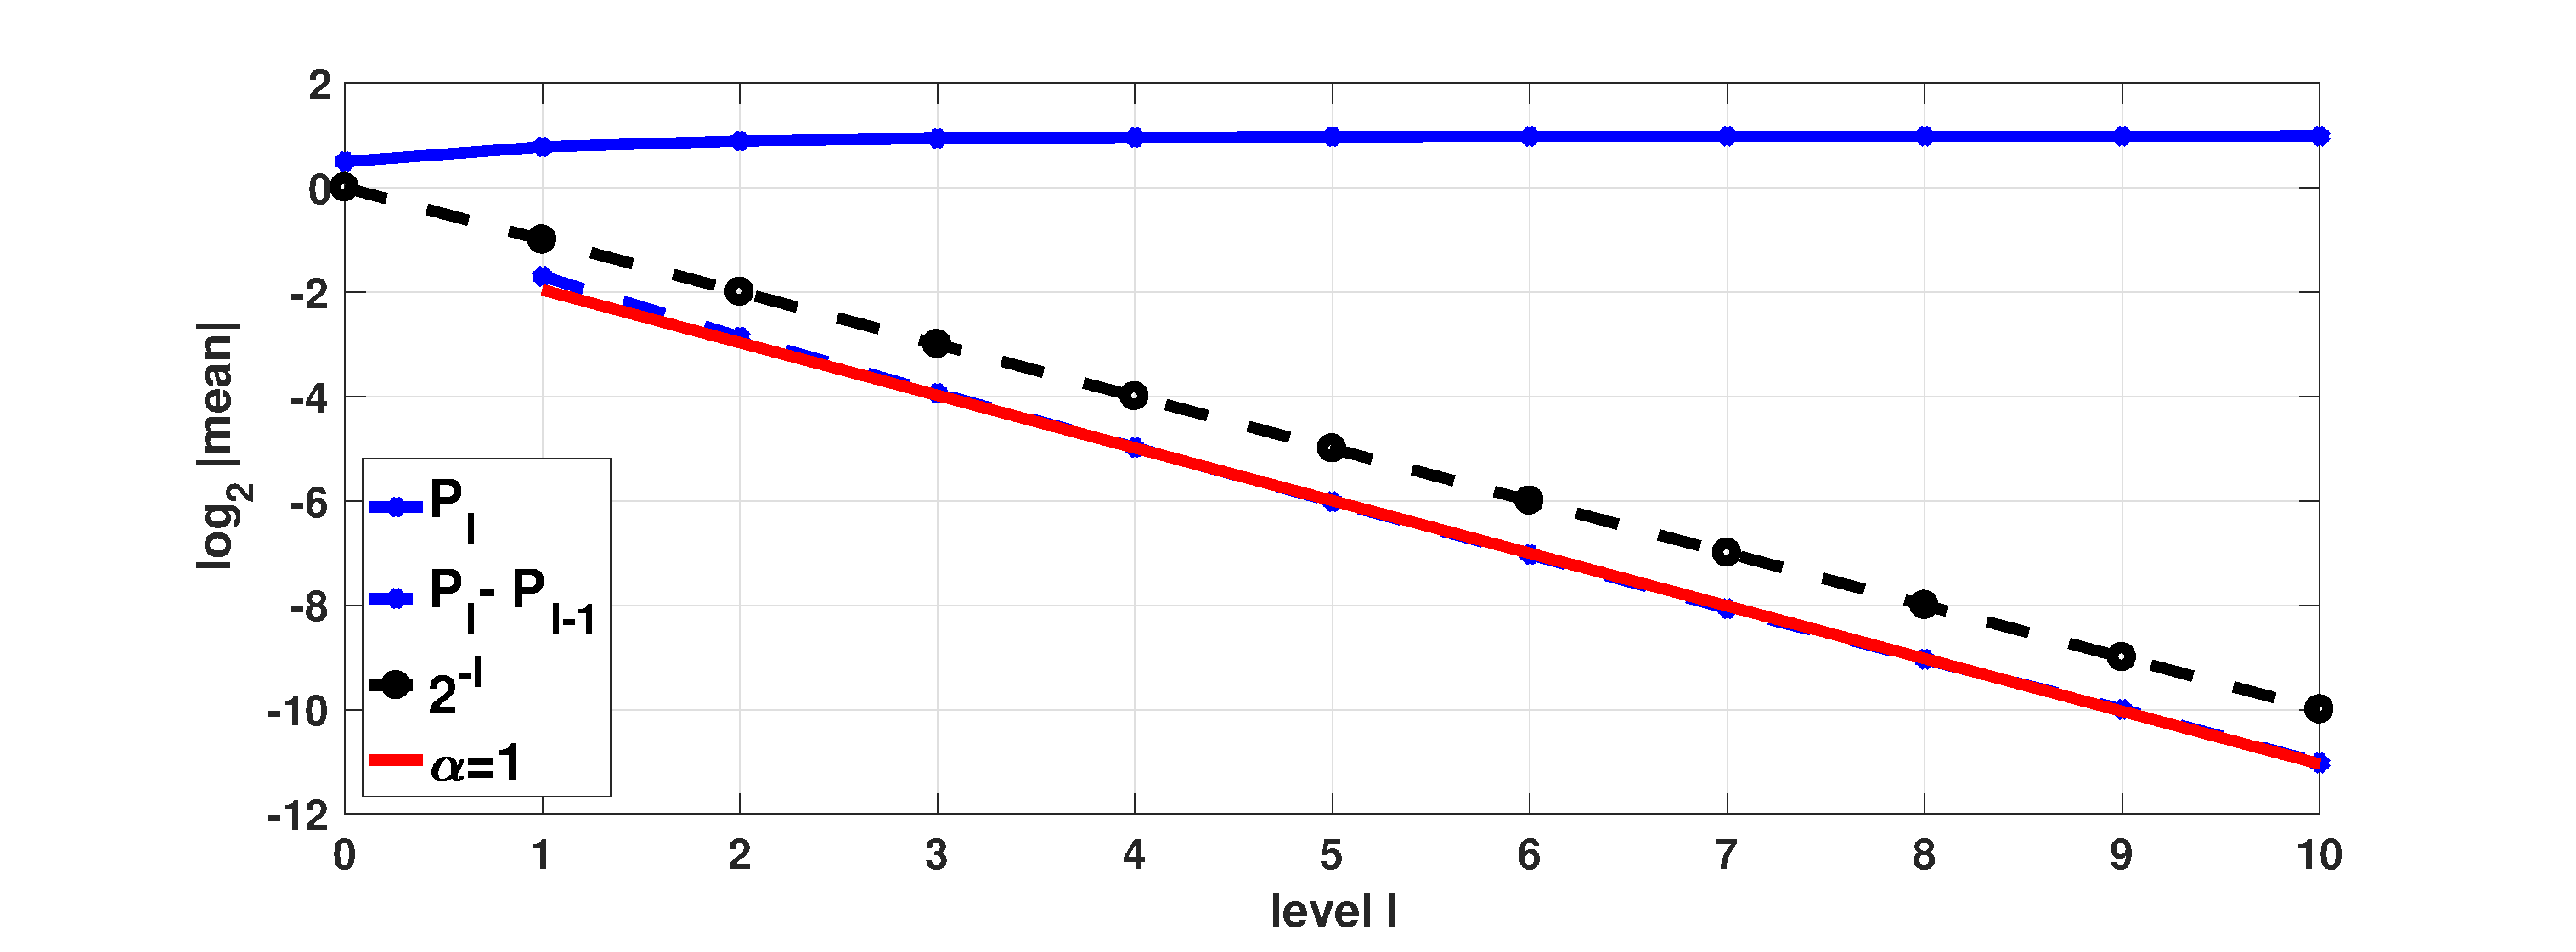
\includegraphics[width=\linewidth]{./figures/MLMC_density_GBM_estimation/density_L0_2_L_10_N_10_5/density_GBM_L_0_2_steps_L_10_N_10_5_weak}
		\caption{}
		\label{fig:GBM_density_weak}
	\end{subfigure}\hfil %% <-- added
	\begin{subfigure}{0.5\textwidth}
		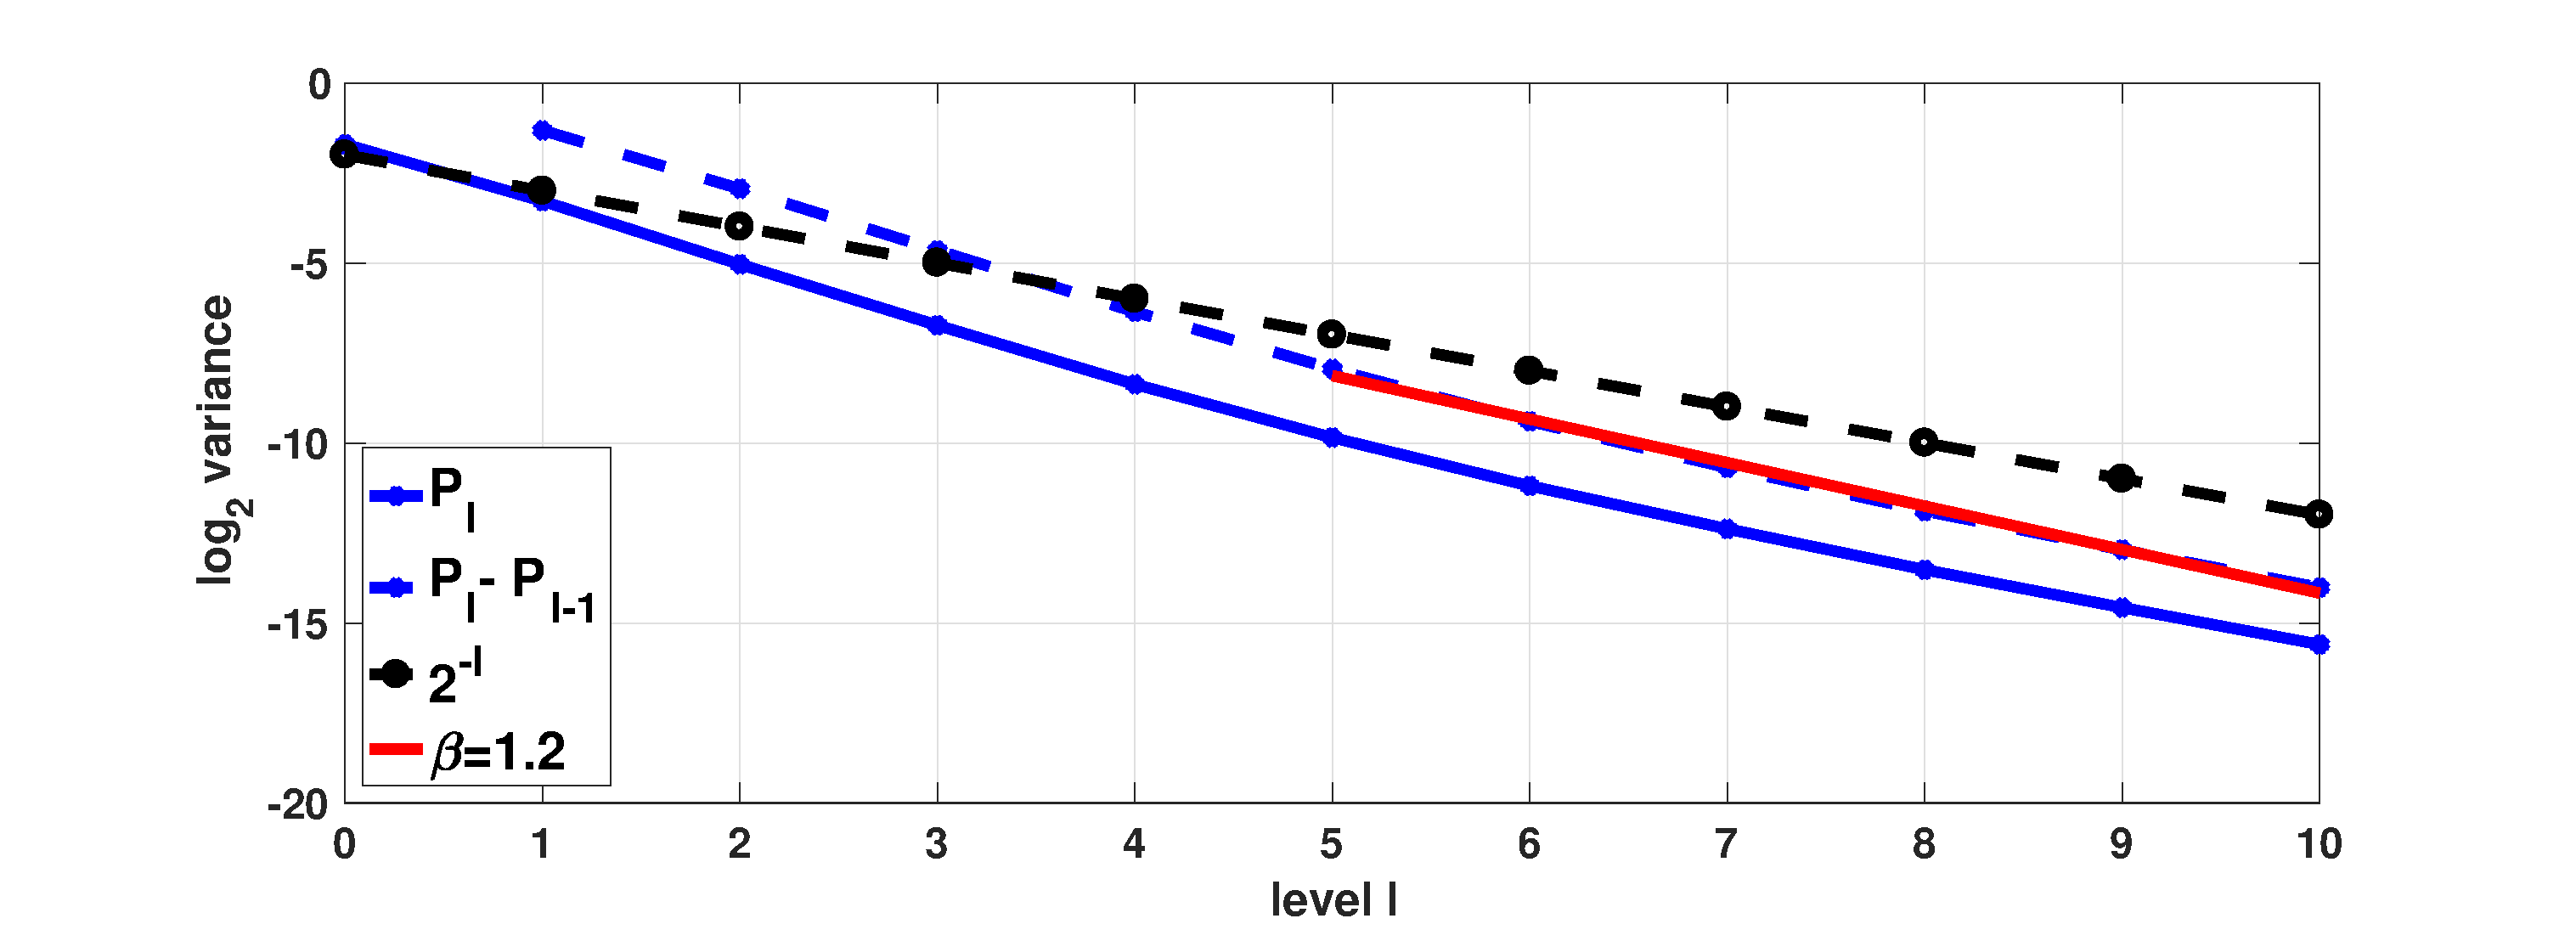
\includegraphics[width=\linewidth]{./figures/MLMC_density_GBM_estimation/density_L0_2_L_10_N_10_5/density_GBM_L_0_2_steps_L_10_N_10_5_strong}
		\caption{}
		\label{fig:GBM_density_strong}
	\end{subfigure}\hfil %% <-- added
	\begin{subfigure}{0.5\textwidth}
		\includegraphics[width=\linewidth]{./figures/MLMC_density_GBM_estimation/density_L0_2_L_10_N_10_5/density_GBM_L_0_2_steps_L_10_N_10_5_kurt}
		\caption{}
		\label{fig:GBM_density_kurt}
	\end{subfigure}
	\caption{Numerical results for  density estimation  using the MLMC method coupled with Euler-Maruyama discretisation of the GBM SDE, after applying  the numerical smoothing. a) Convergence of  the weak error, $\expt{P_{\ell}-P_{\ell-1}}$, b) Convergence of  the strong error, $\text{Var}\left[P_{\ell}-P_{\ell-1}\right]$, c) the kurtosis $\kappa_{L}$, defined in \eqref{eq:Kurtosis}.  Estimation done with $M=10^6$ samples.}
	\label{fig:outputs_GBM_density}	
\end{figure}
\FloatBarrier

	\begin{figure}[h!]
\centering
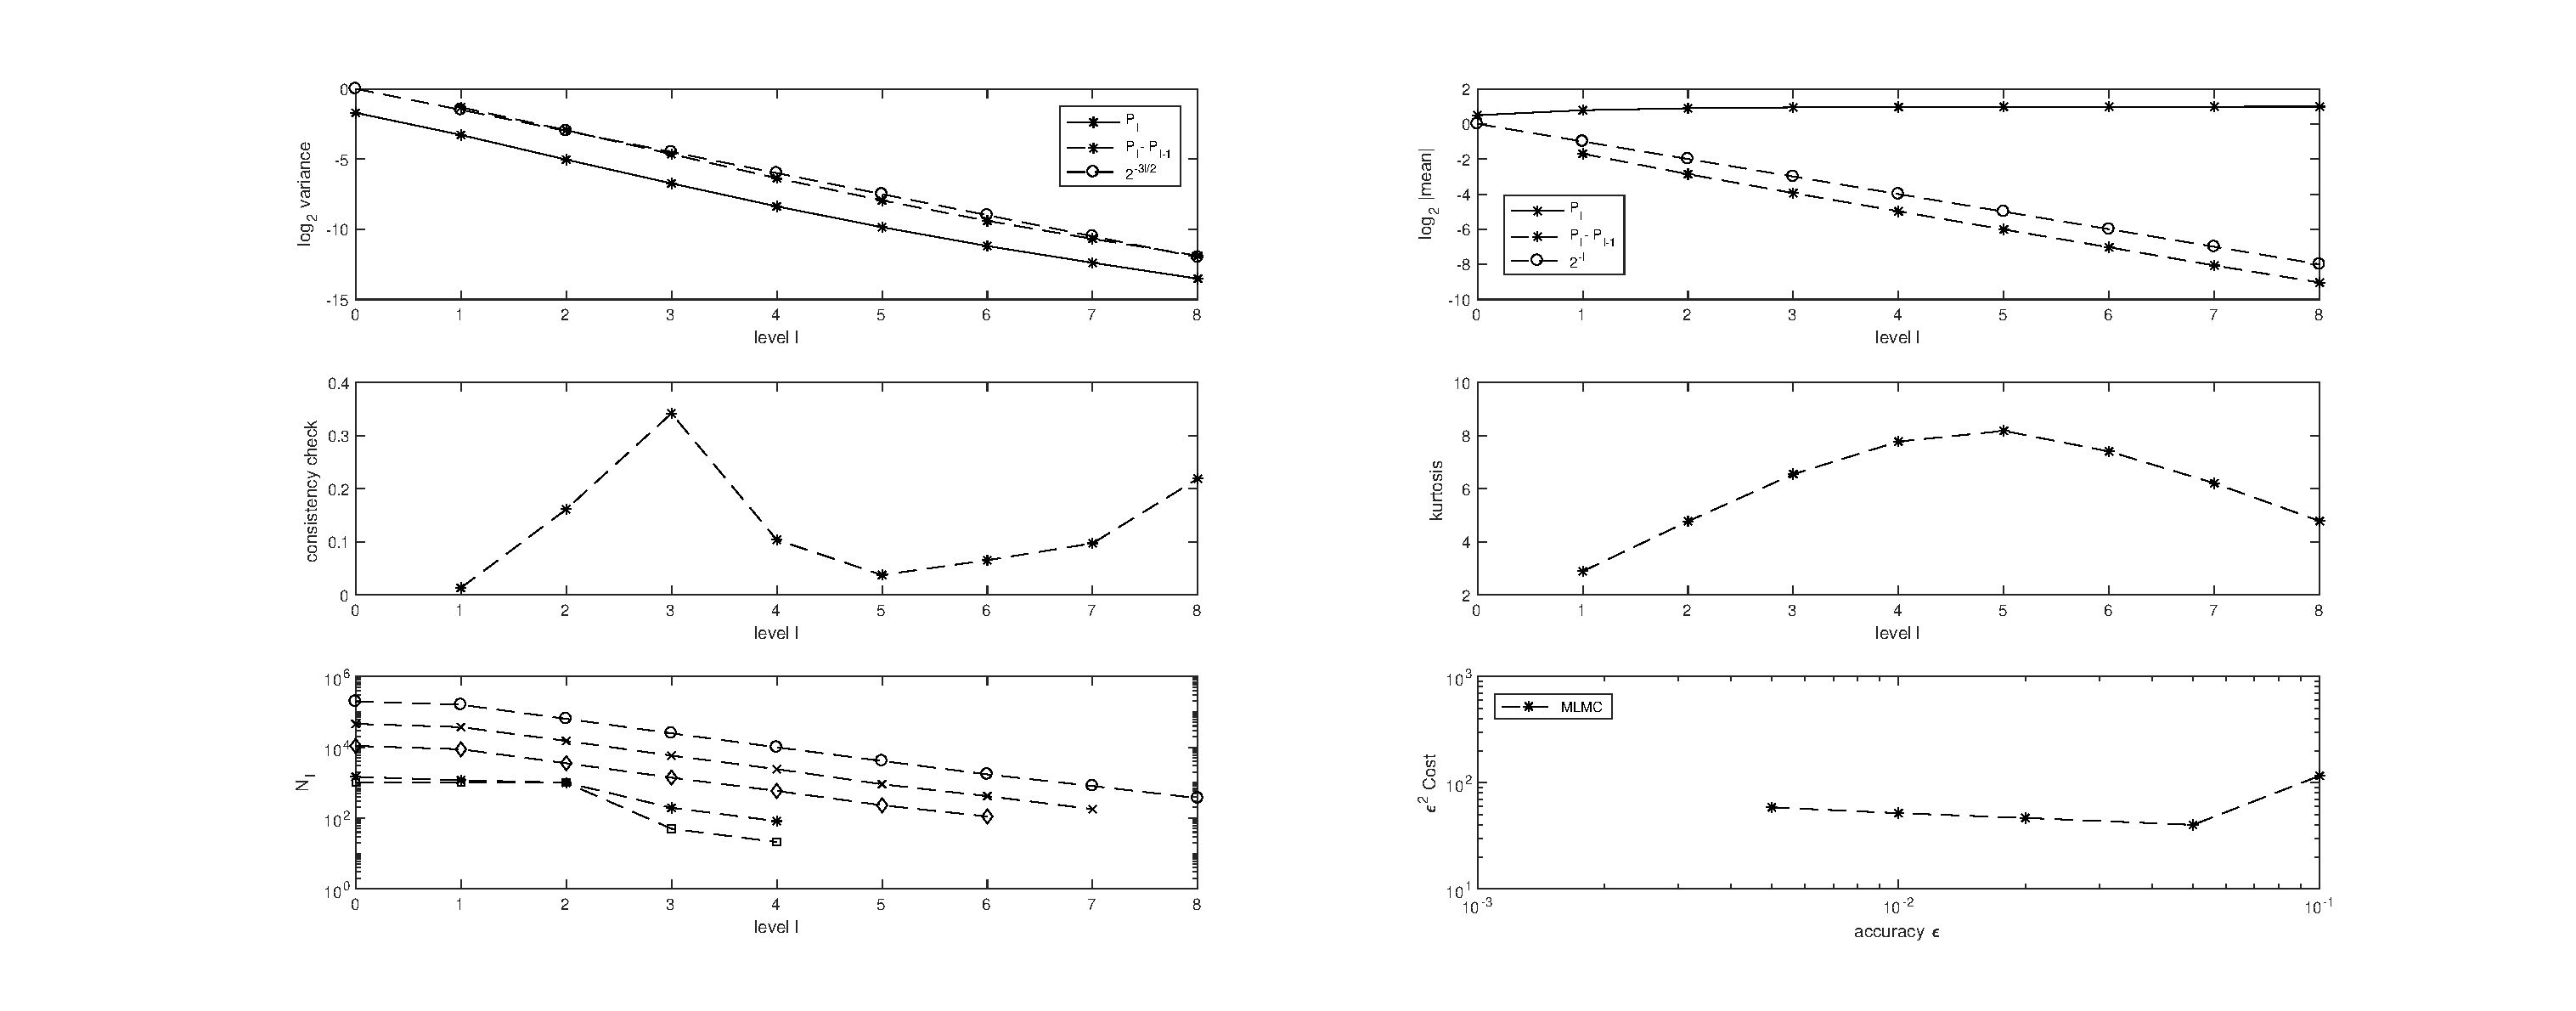
\includegraphics[width=1.2\linewidth]{./figures/MLMC_density_GBM_estimation/density_L0_2_L_8.eps}

\caption{Numerical results for  density estimation  using the MLMC method coupled with Euler-Maruyama discretisation of the GBM SDE, after applying  the numerical smoothing. We mention that observing a decaying variance of $P_{\ell}$ here is expected since we used Brownian bridge for path construction, and the QoI depends only on the terminal value of the Brownian bridge which has a variance scaled of order $\Delta t$.}
\label{fig:euler_density_MLMC_with_smoothing}
\end{figure}
\FloatBarrier
We emphasize that our approach can be extended in a straightforward manner to any kind of dynamics, since it is based on numerical smoothing based on solving a root finding problem.  In the following Section, we show the advantage of our approach for the Heston model where discretization of the asset price is indeed needed.

\subsubsection{Approximating density under the Heston model}\label{sec:Approximating density under the Heston model}
%Since the asset price in the  Heston model (see \eqref{eq:dynamics Heston})   has similar structure of dynamics compared to the GBM with the difference of the volatility being non constant, we can show also that 
%\begin{align}
%\rho_{X}(u)&=\expt{\delta(X-y)}\nonumber\\
%&=\exp\left(-(y^\ast(u))^2/2\right) \frac{d y^\ast}{dx}(u),
%\end{align}
%where $y^\ast(K)$ is the kink location obtained by solving numerically 
%$$X(T; y^\ast(K), \mathbf{z}_{-1})=K,$$
%where  $\mathbf{z}$ is $2N-1$ Gaussian random  vector ($N$ is the number of time steps) used for Brownian bridge construction.

As an illustration, we choose to compute the density $\rho_{X}$  such that $X$ is a Heston asset with parameters: $S_0=K=1$, $v_0=0.04$, $\mu=0$,  $\rho=-0.9$, $\kappa=1$, $\xi=0.1$, $\theta=0.0025$.  In Figures \ref{fig:Heston_density_MLMC_with_smoothing_OU} and \ref{fig:Heston_density_MLMC_with_smoothing_FT}, we show the numerical results  for computing the $\rho_{X}$ at $u=1$, using  MLMC coupled with the numerical smoothing idea. From Figures \ref{fig:Heston_density_MLMC_with_smoothing_OU} and \ref{fig:Heston_density_MLMC_with_smoothing_FT}, we can check that we obtain a strong convergence rate of order $1/2$ (see  top left plot in Figure \ref{fig:Heston_density_MLMC_with_smoothing_OU} and \ref{fig:Heston_density_MLMC_with_smoothing_FT}), which results in a complexity of the MLMC estimator to be of order $TOL^{-2.5}$, where $TOL$ is a prescribed tolerance.

\begin{figure}[htb]
	\centering % <-- added
	\begin{subfigure}{0.5\textwidth}
		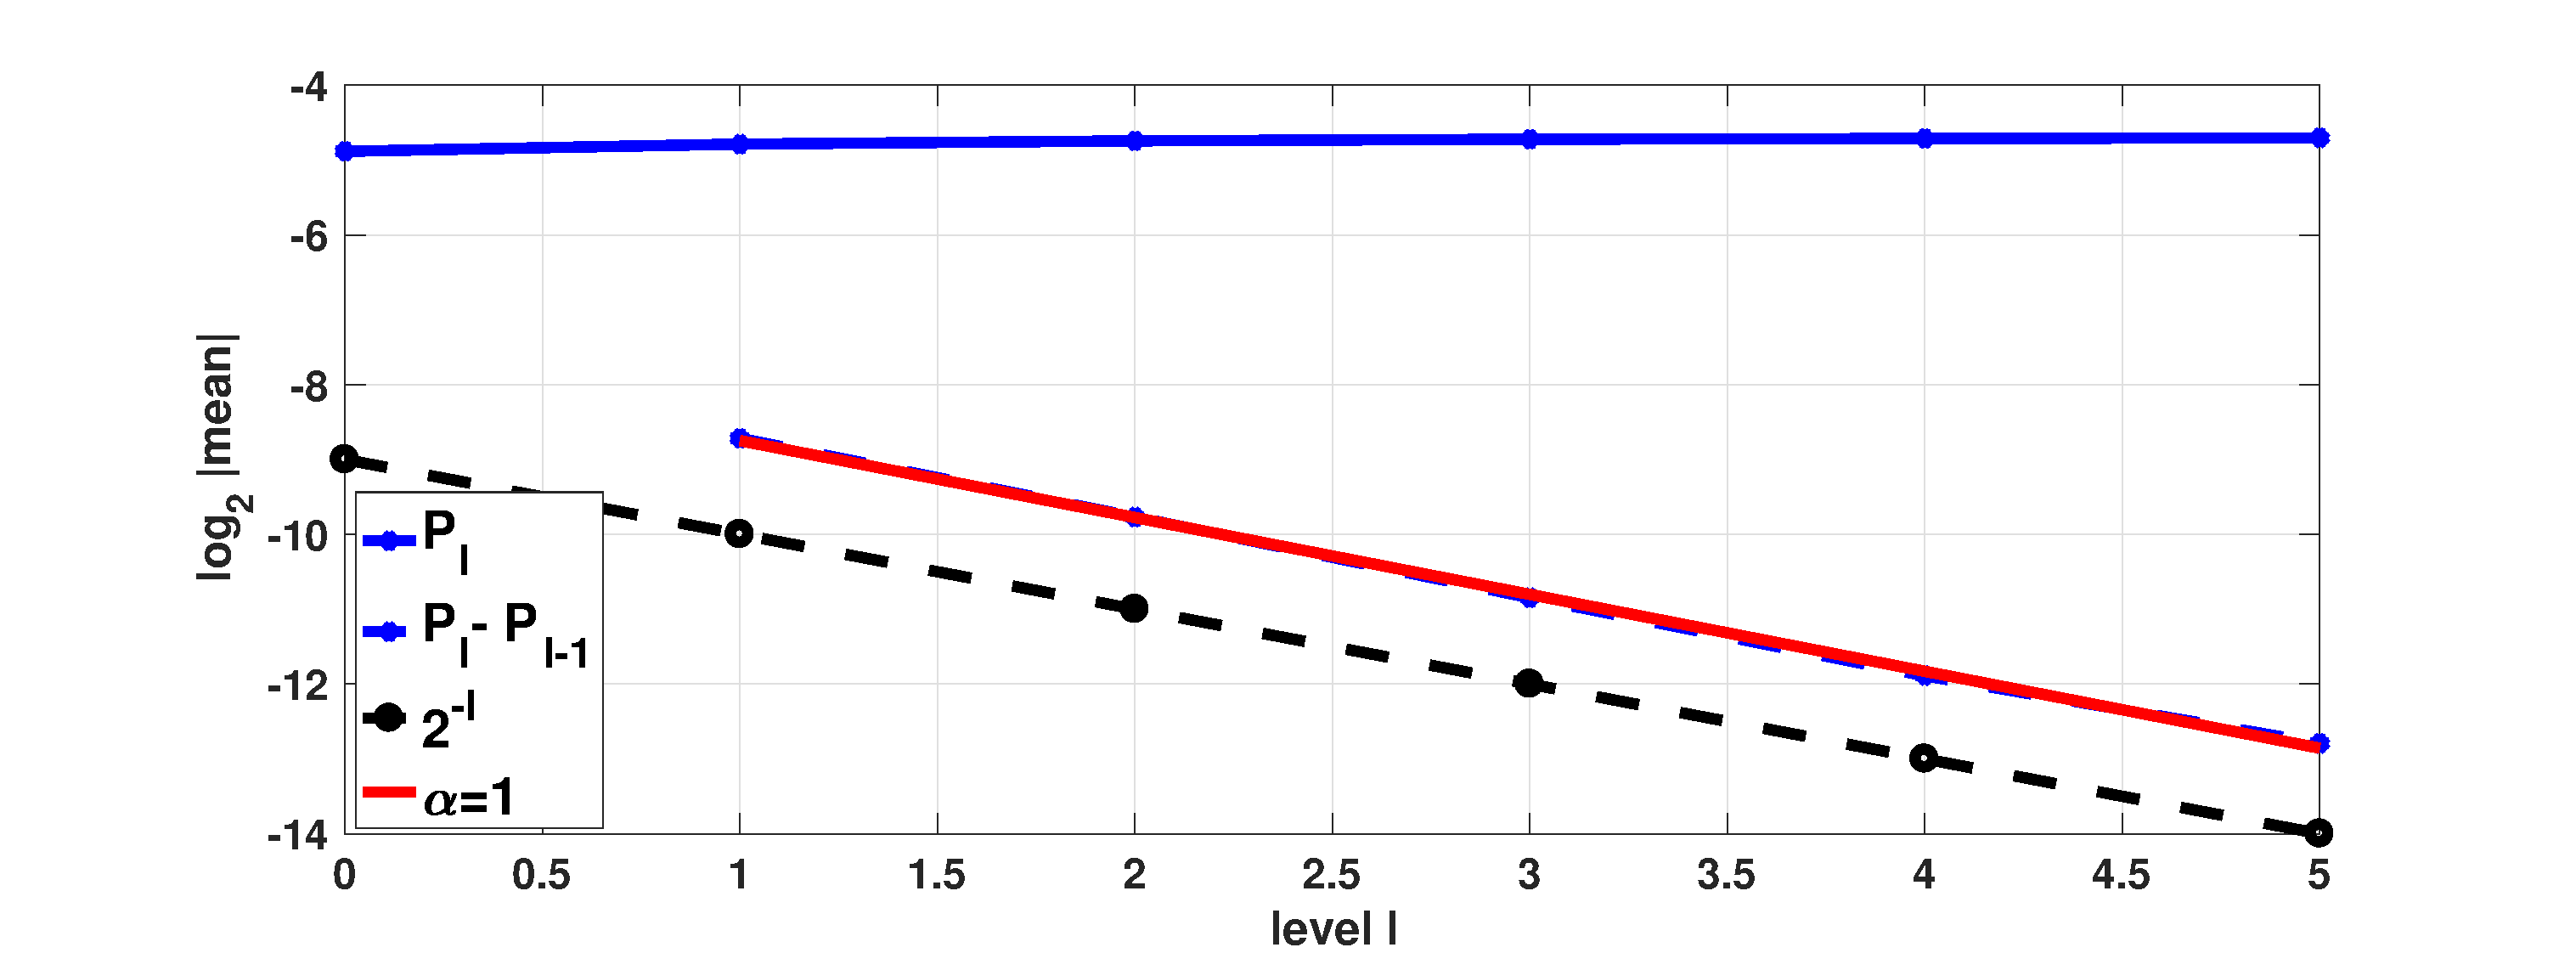
\includegraphics[width=\linewidth]{./figures/MLMC_density_Heston_estimation/OU/density_option_set1_L_0_4_steps_L_6_N_10_6_beta_32/density_option_set1_L_0_2_steps_L_6_N_10_6_weak}
		\caption{}
		\label{fig:hest_density_weak}
	\end{subfigure}\hfil %% <-- added
	\begin{subfigure}{0.5\textwidth}
		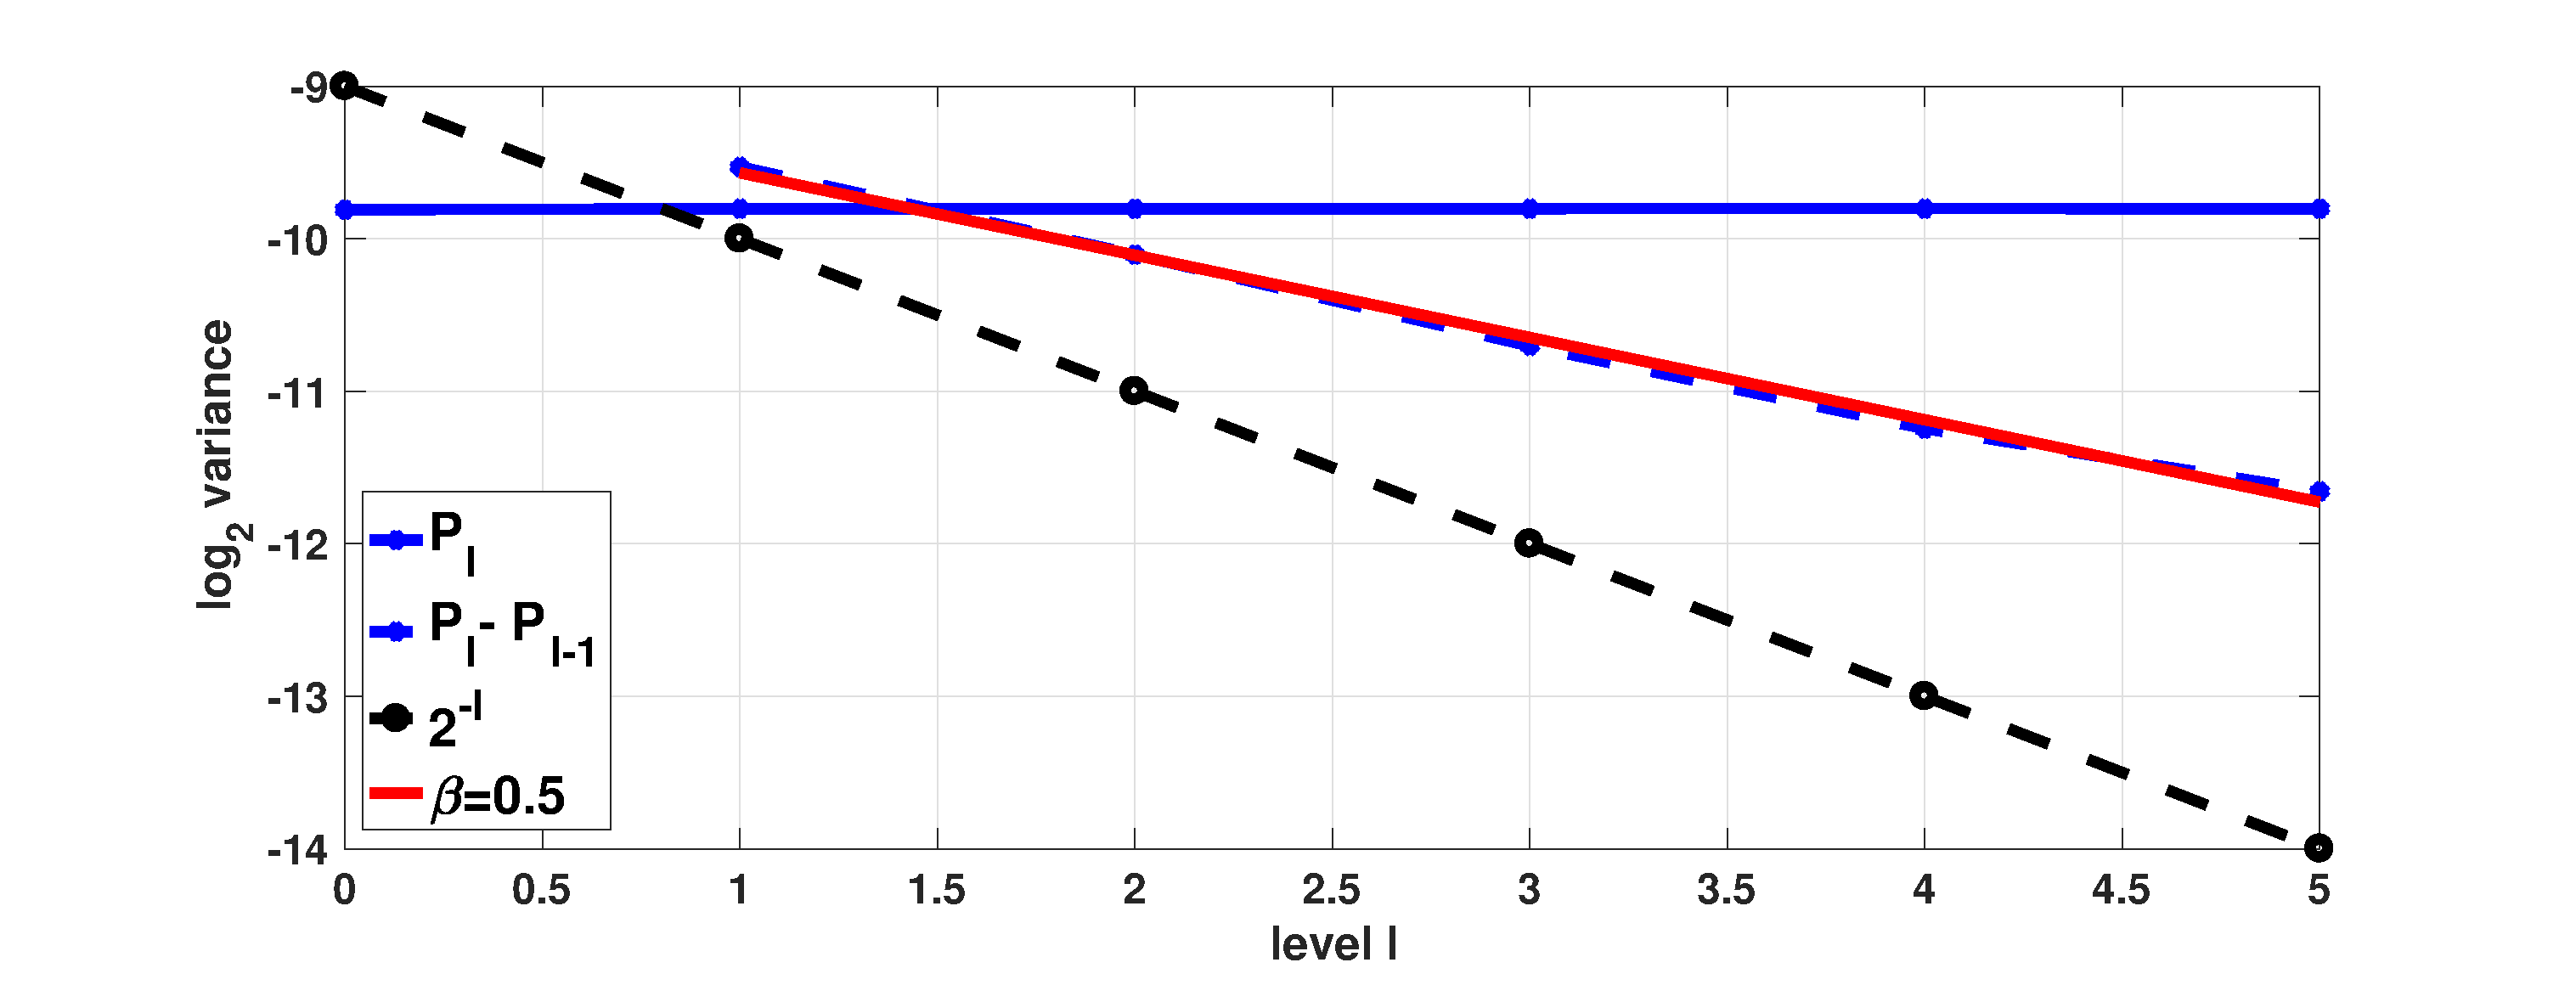
\includegraphics[width=\linewidth]{./figures/MLMC_density_Heston_estimation/OU/density_option_set1_L_0_4_steps_L_6_N_10_6_beta_32/density_option_set1_L_0_2_steps_L_6_N_10_6_strong}
		\caption{}
		\label{fig:hest_density_strong}
	\end{subfigure}\hfil %% <-- added
	\begin{subfigure}{0.5\textwidth}
		\includegraphics[width=\linewidth]{./figures/MLMC_density_Heston_estimation/OU/density_option_set1_L_0_2_steps_L_5_N_10_5/density_option_set1_L_0_2_steps_L_5_N_10_5_kurt}
		\caption{}
		\label{fig:hest_density_kurt}
	\end{subfigure}
	\caption{Numerical results for  density estimation  for Heston model using the MLMC method coupled with  the smooth   scheme in Section \ref{sec:Discretization of Heston model with the volatility process Simulated using the sum of  Ornstein-Uhlenbeck (Bessel) processes}, and with smoothing of the payoff. a) Convergence of  the weak error, $\expt{P_{\ell}-P_{\ell-1}}$, b) Convergence of  the strong error, $\text{Var}\left[P_{\ell}-P_{\ell-1}\right]$, c) the kurtosis $\kappa_{L}$, defined in \eqref{eq:Kurtosis}.  Estimation done with $M=10^6$ samples.}
	\label{fig:outputs_heston_density_OU}	
\end{figure}
\FloatBarrier

	\begin{figure}[h!]
\centering
\includegraphics[width=1.2\linewidth]{./figures/MLMC_density_Heston_estimation/OU/digital_option_set1_L_0_8_steps_L_5.eps}

\caption{Numerical results for  density estimation  for Heston model using the MLMC method coupled with  the smooth   scheme in Section \ref{sec:Discretization of Heston model with the volatility process Simulated using the sum of  Ornstein-Uhlenbeck (Bessel) processes}, and with smoothing of the payoff.}
\label{fig:Heston_density_MLMC_with_smoothing_OU}
\end{figure}


\FloatBarrier

\begin{figure}[htb]
	\centering % <-- added
	\begin{subfigure}{0.5\textwidth}
		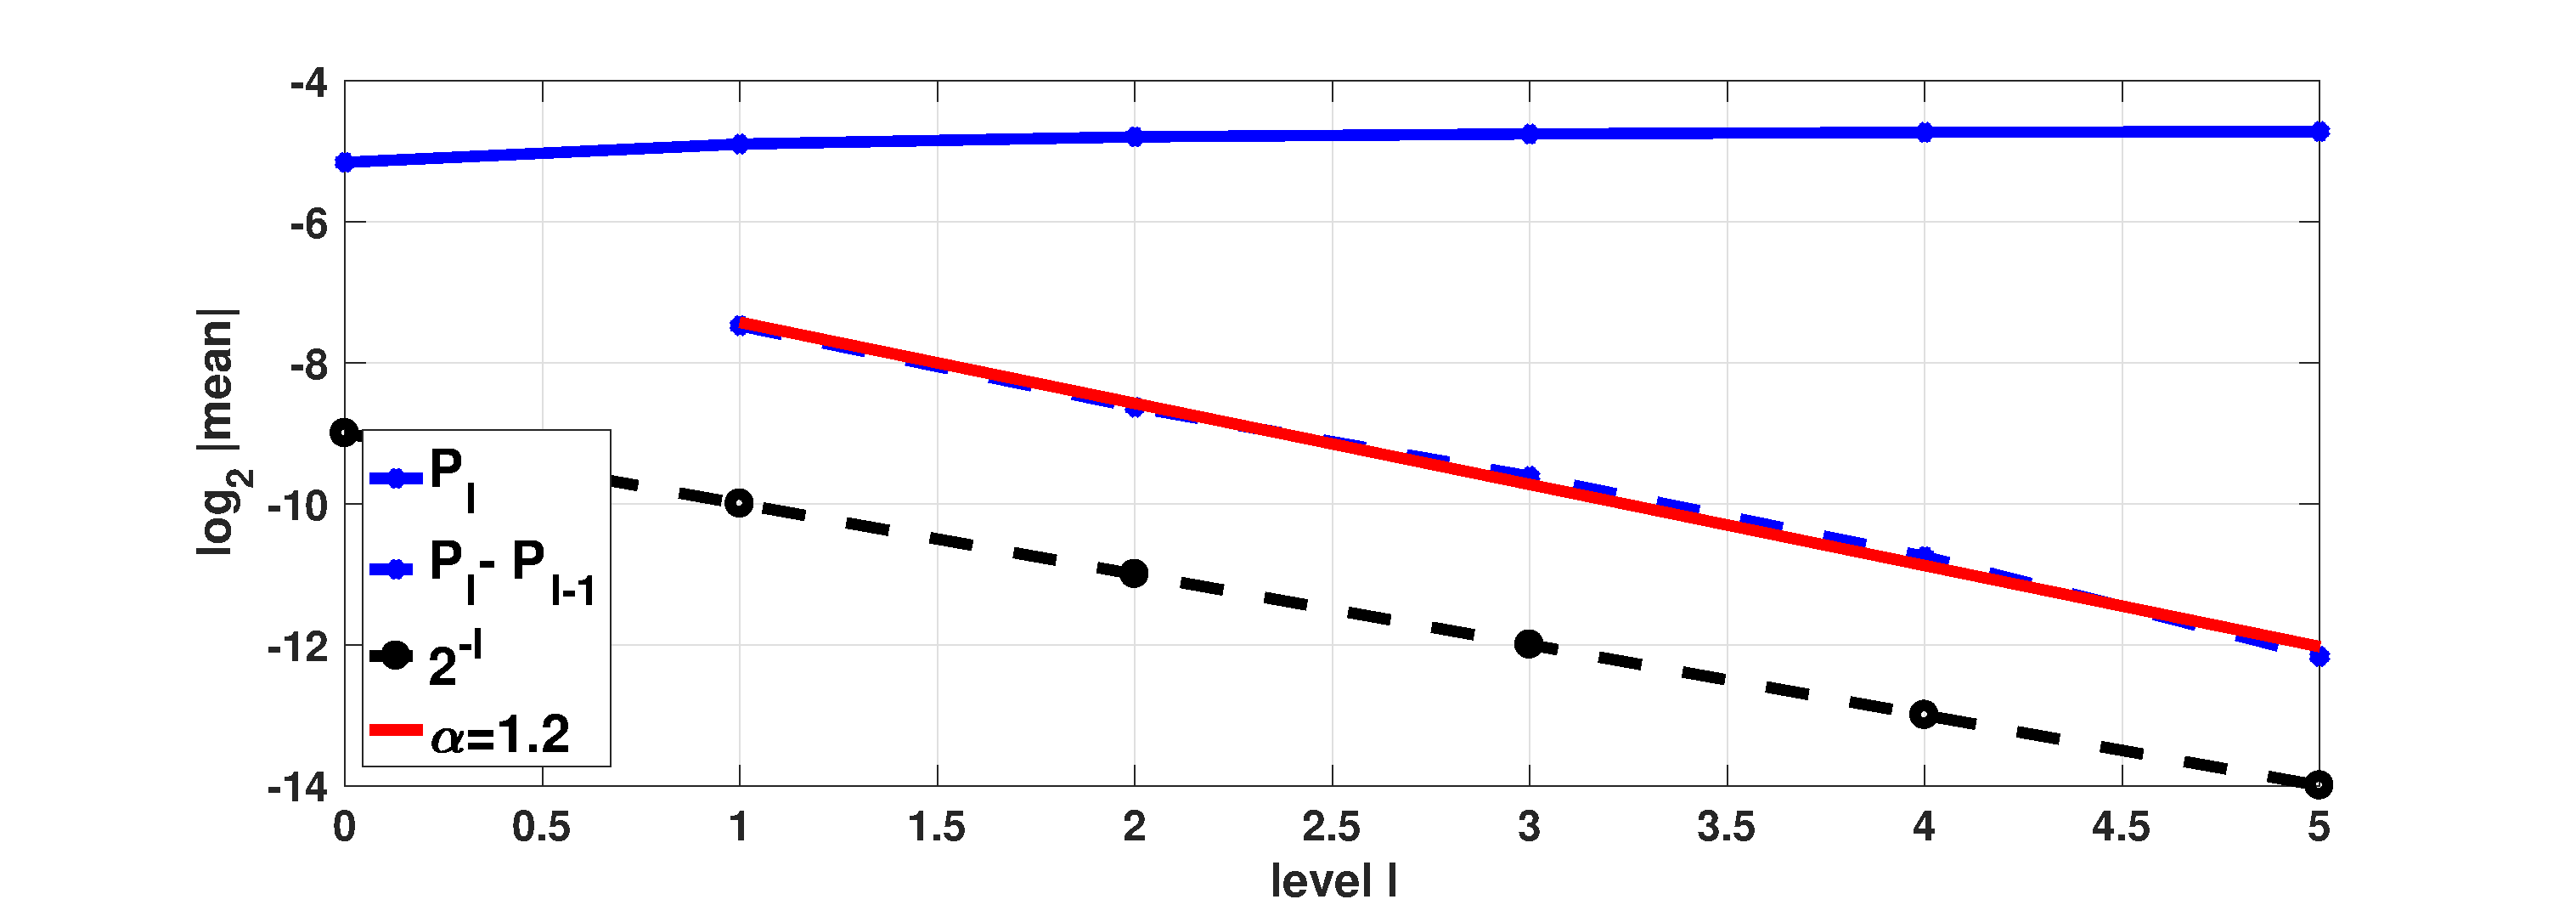
\includegraphics[width=\linewidth]{./figures/MLMC_density_Heston_estimation/FT/density_option_set1_L_0_2_steps_L_5_N_10_5_bet_32/density_option_set1_L_0_2_steps_L_5_N_10_5_weak}
		\caption{}
		\label{fig:hest_density_weak_FT}
	\end{subfigure}\hfil %% <-- added
	\begin{subfigure}{0.5\textwidth}
		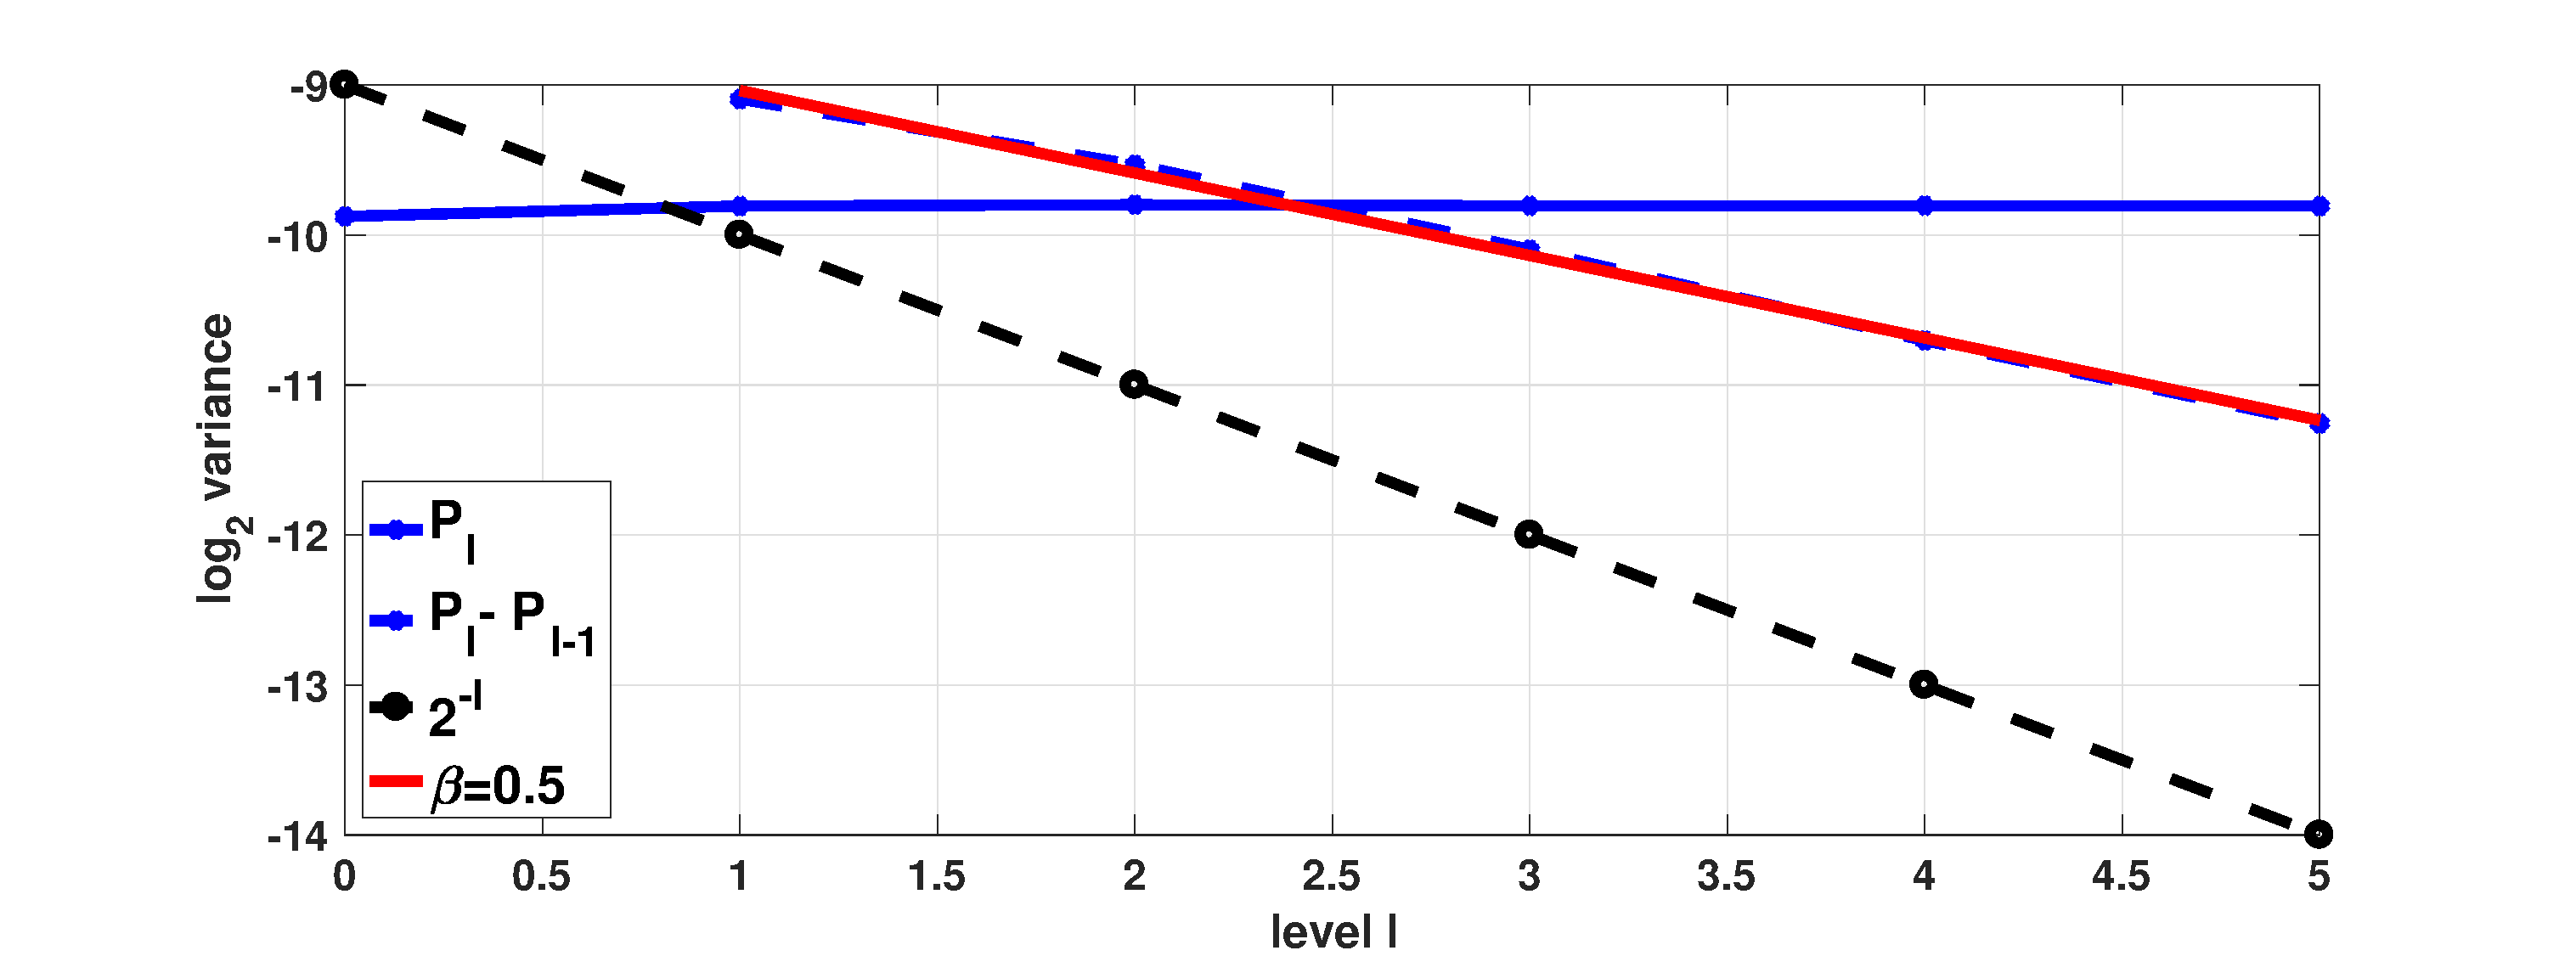
\includegraphics[width=\linewidth]{./figures/MLMC_density_Heston_estimation/FT/density_option_set1_L_0_2_steps_L_5_N_10_5_bet_32/density_option_set1_L_0_2_steps_L_5_N_10_5_strong}
		\caption{}
		\label{fig:hest_density_strong_FT}
	\end{subfigure}\hfil %% <-- added
	\begin{subfigure}{0.5\textwidth}
		\includegraphics[width=\linewidth]{./figures/MLMC_density_Heston_estimation/FT/density_option_set1_L_0_2_steps_L_5_N_10_5_bet_32/density_option_set1_L_0_2_steps_L_5_N_10_5_kurt}
		\caption{}
		\label{fig:hest_density_kurt_FT}
	\end{subfigure}
	\caption{Numerical results for  density estimation  for Heston model  using the MLMC method coupled with   the Full truncation scheme in Section \ref{sec:Discretization of Heston model with a non smooth transformations for the volatility process} , and with smoothing of the payoff. a) Convergence of  the weak error, $\expt{P_{\ell}-P_{\ell-1}}$, b) Convergence of  the strong error, $\text{Var}\left[P_{\ell}-P_{\ell-1}\right]$, c) the kurtosis $\kappa_{L}$, defined in \eqref{eq:Kurtosis}.  Estimation done with $M=10^5$ samples.}
	\label{fig:outputs_heston_density_FT}	
\end{figure}
\FloatBarrier
	\begin{figure}[h!]
\centering
\includegraphics[width=1.2\linewidth]{./figures/MLMC_density_Heston_estimation/FT/digital_option_set1_L_0_8_steps_L_5.eps}

\caption{Numerical results for  density estimation  for Heston model  using the MLMC method coupled with   the Full truncation scheme in Section \ref{sec:Discretization of Heston model with a non smooth transformations for the volatility process} , and with smoothing of the payoff.}
\label{fig:Heston_density_MLMC_with_smoothing_FT}
\end{figure}
\FloatBarrier


\begin{remark}
Although we just illustrated the benefit of our approach when coupled with MLMC for computing the density  of the asset price under the GBM dynamics (Section \ref{sec:Approximating density under the GBM model}) and Heston dynamics (Section \ref{sec:Approximating density under the Heston model}), we emphasize that it can be easily extended to any kind of model dynamics. Furthermore, our approach can be easily extended to computing Greeks of a digital options, involving the delta functions.
\end{remark}
